% arara: clean: {
% arara: --> extensions:
% arara: --> ['aux','bbl','bcf','blg','log','out','run.xml','toc','pdf']
% arara: --> }
% arara: lualatex: {
% arara: --> shell: no,
% arara: --> draft: yes,
% arara: --> interaction: batchmode
% arara: --> }
% arara: biber
% arara: lualatex: {
% arara: --> shell: no,
% arara: --> draft: yes,
% arara: --> interaction: batchmode
% arara: --> }
% arara: lualatex: {
% arara: --> shell: no,
% arara: --> draft: no,
% arara: --> interaction: batchmode
% arara: --> }
% arara: clean: {
% arara: --> extensions:
% arara: --> ['aux','bbl','bcf','blg','log','out','run.xml','toc']
% arara: --> }
\documentclass[a4paper]{amsart}

\usepackage[svgnames]{xcolor}
\usepackage{graphicx}

\newenvironment{proofs}{\paragraph{Proof:}}{\hfill$\square$}

\usepackage[ngerman,english]{babel}

\usepackage{mathtools}
\usepackage[ISO]{diffcoeff}
\usepackage{dsfont}

\graphicspath{{images/}}

\let\oldforall\forall
\renewcommand{\forall}{\oldforall \, }
\let\oldexist\exists
\renewcommand{\exists}{\oldexist \: }
\newcommand\existu{\oldexist! \: }

\usepackage[
	% citestyle=numeric,
	% style=amsplain,
	% backend=biber,
	% defernumbers=true,
	% sorting=ynt,
	% maxcitenames=4
]{biblatex}
\addbibresource{references.bib}

\usepackage[
	pdfencoding=auto,
	linktocpage=true,
	colorlinks=true,
	linkcolor=blue,
	urlcolor=magenta,
	pdfpagelabels
	%	bookmark=false
]{hyperref}

\title{The Stone – Weierstraß Theorem}
\author{Carlos Aznarán Laos}
\date{\today}
\usepackage{beamerarticle}
\setjobnamebeamerversion{main.beamer}

\begin{document}

\mode<article>{ % all
	\begin{frame}
	\maketitle

	\note{
		Comment a little about the life of

		\begin{itemize}
			\item

			      Karl Theodor Wilhelm Weierstraß
			      (31. Oktober 1815 in Münsterland; † 19. Februar 1897 in Berlin).
			      On the \alert{top right}.

			\item

			      Marshall Harvey Stone
			      (April 8, 1903 - January 9, 1989).
			      On the \alert{below right}.

			\item


			      Lipót Fejér
			      (9 February 1880 - 15 October 1959).
			      On the \alert{left}.
		\end{itemize}

		\

		The slides were a part of final project of functional analysis
		course with professor Manuel Toribio Cangana in 2022.

		\

		Explain in a single sentence the importance of approximation
		theorems.

		\

		About me: .

		\

		Some facts: is my favourite theorem.

		\

		Applications in numerical analysis, neural networks.
	}
\end{frame}

	\begin{abstract}
		We.
	\end{abstract}

	% \begin{frame}
	\frametitle{\contentsname}

	\tableofcontents
	\begin{picture}(0,0)
		\put(420,200){\makebox(0,0)[rt]{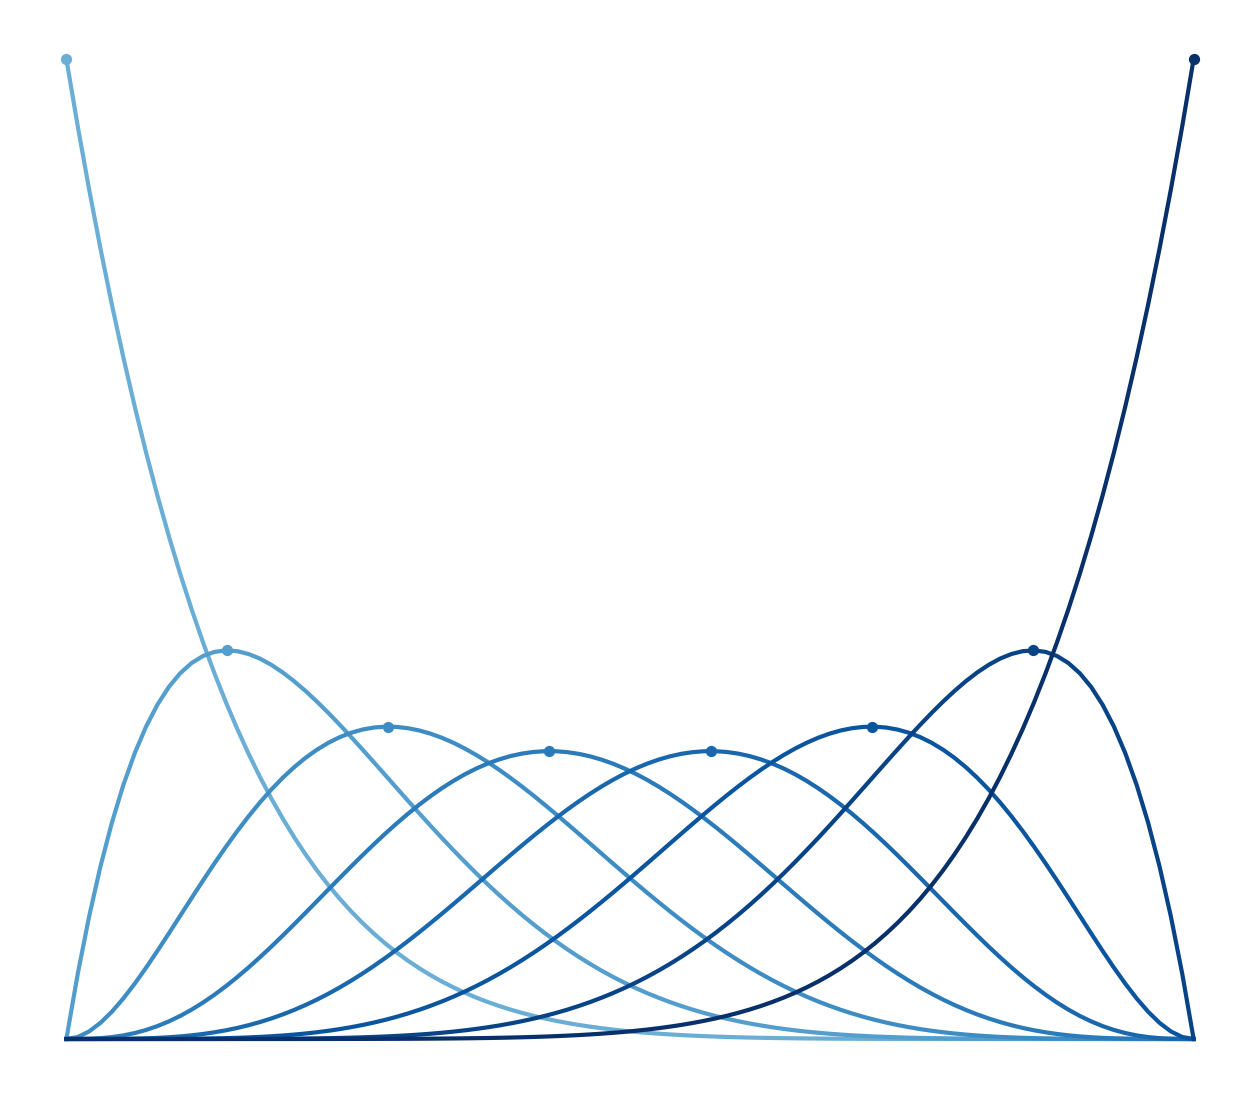
\includegraphics[width=0.5\paperwidth]{bernstein}}}
	\end{picture}

	\note{
		The talk is divided in five sections.

		\

		\begin{enumerate}
			\item

			      We will show the objectives.

			\item

			      We will show a lot of definitions.

			\item

			      We will develop lemmas and the proof of approximation theorem.

			\item

			      In the fourth one, we will stablish the title's theorem.

			\item

			      In the fifth one, we will show some theoretical applications and simulations.
			      For example, the universal approximation.
		\end{enumerate}

		\

		Feel free to ask anytime.

		\

		Let's start!
	}
\end{frame}
	\tableofcontents
	%\section{Objectives}

\begin{frame}
	\frametitle{\secname}
	\begin{columns}
		\begin{column}{0.38\textwidth}
			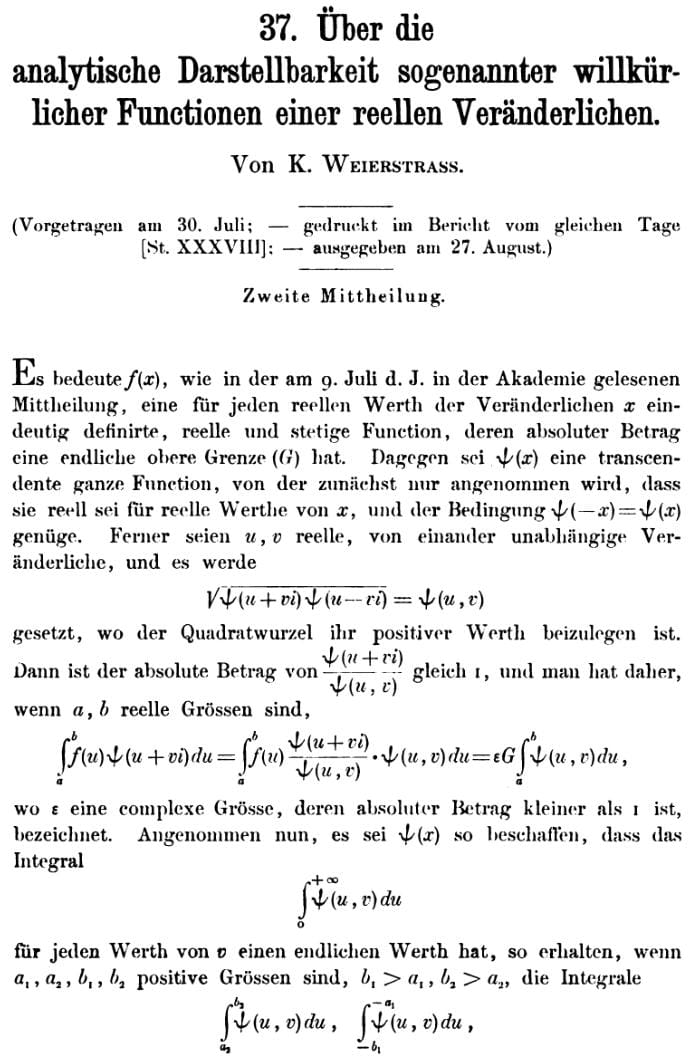
\includegraphics[width=0.3\paperwidth]{original_approximation}
		\end{column}
		\begin{column}{0.58\textwidth}
			\begin{itemize}
				\item

				      Weierstraß proved the \alert{approximation theorem} at
				      the age of 70.
				      He used the \alert{Weierstraß transform}~\cite{
					      weierstrass1885,
					      Schep2007
				      }.

				      \fcolorbox{DarkBlue}{yellow}{
					      \begin{math}
						      \displaystyle
						      \forall f\in C\left(\mathds{R},\mathds{R}\right):
						      F\left(\theta\right)=
						      \frac{1}{\sqrt{4\pi}}
						      \int\limits_{-\infty}^{\infty}
						      f\left(y\right)
						      \exp\left(
						      -\frac{\left(\theta-y\right)^{2}}{4}
						      \right)\dl y.
					      \end{math}
				      }

				\item

				      In 1912, Bernstein made a direct proof with the
				      \alert{Bernstein polynomial}~\cite{Saha2021}.

				\item

				      Proof the \alert{Fejér's theorem}~\cite{Fejér1903}.

				\item

				      Proof the \alert{Stone – Weierstraß theorem} in the
				      real, complex, quaternion and locally compact versions.

				\item

				      Proof the \alert{Bishop's theorem}~\cite{Rudin1991}.
			\end{itemize}
		\end{column}
	\end{columns}

	\note{
		A little of story, Weierstraß was interested in the heat
		equation, he develop la Weierstraß transform.

		\

		.
	}
\end{frame}
	\section{Introduction}

\begin{frame}
	\frametitle{\secname}
	.
\end{frame}
	\section{Preliminaries}

\mode*
In the presentation of the material we mostly
follow~\cite{Axler2020,Simon2015,Rodriguez2021}.

\mode<all>
\begin{frame}
	\frametitle{\secname}

	\begin{definition}[Topological space]
		Let $X$ be a set.
		A \alert{topology} on $X$ is a family $\mathcal{T}\subset 2^{X}$
		that holds

		\begin{columns}
			\begin{column}{0.48\textwidth}
				\begin{itemize}
					\item

					      \begin{math}
						      \forall\left\{A_{i}\right\}_{i=1}^{n}\subset
						      \mathcal{T}\implies
						      \bigcap\limits_{i=1}^{n}
						      A_{i}\in\mathcal{T}
					      \end{math}.
				\end{itemize}
			\end{column}
			\begin{column}{0.48\textwidth}
				\begin{itemize}
					\item

					      \begin{math}
						      \forall
						      \left\{
						      A_{\lambda}
						      \right\}_{\lambda\in\Lambda}\subset
						      \mathcal{T}\implies
						      \bigcup\limits_{\lambda\in\Lambda}
						      A_{\lambda}\in\mathcal{T}
					      \end{math}.
				\end{itemize}
			\end{column}
		\end{columns}

		If $\mathcal{T}$ is a topology on $X$, then
		$\left(X,\mathcal{T}\right)$ is a \alert{topological space}.
		The sets in $\mathcal{T}$ are \alert{open sets}.
	\end{definition}

	\begin{definition}[Open cover]
		Let $\left(X,\mathcal{T}\right)$ be a topological space.
		$\mathcal{C}\subset\mathcal{T}$ is an \alert{open cover}
		of $X$ iff
		\begin{math}
			X\subseteq\bigcup\limits_{A\in\mathcal{C}}A
		\end{math}.
	\end{definition}

	\begin{definition}[Hausdorff topological space or $T_{2}$]
		A topological space $\left(X,\mathcal{T}\right)$ is
		\alert{Hausdorff} iff $\forall x,y\in X,x\neq y$:
		$\exists U,V\in\mathcal{T}$ such that
		\begin{math}
			\forall x\in U, y\in V:
			U\cap V=\emptyset
		\end{math}.
	\end{definition}

	\begin{definition}[Compact topological space]
		A topological space $\left(X,\mathcal{T}\right)$ is
		\alert{compact} iff each open cover of $X$ has a finite subcover.
	\end{definition}

	\note{
		Examples of
		\begin{description}
			\item[Hausdorff space]

				.

			\item[Compact space]

				.
		\end{description}

		\

		Examples of non

		\begin{description}
			\item[Hausdorff space]

				.

			\item[Compact space]

				.
		\end{description}

		\

		Some facts of

		\begin{description}
			\item[Hausdorff space]

				.

			\item[Compact space]

				.
		\end{description}
	}
\end{frame}
\begin{frame}
	\frametitle{\secname}

	\begin{definition}[$\sigma$-algebra]
		Let $X$ be a set.
		A \alert{$\sigma$-algebra} on $X$ is a family
		$\mathcal{F}\subset 2^{X}$ that holds

		\begin{columns}
			\begin{column}{0.48\textwidth}
				\begin{itemize}
					\item

					      \begin{math}
						      \forall A\in\mathcal{F}\implies
						      X\setminus A\in\mathcal{F}
					      \end{math}.
				\end{itemize}
			\end{column}
			\begin{column}{0.48\textwidth}
				\begin{itemize}
					\item

					      \begin{math}
						      \forall
						      \left\{A_{i}\right\}_{i\in\mathds{N}}\subset
						      \mathcal{F}\implies
						      \bigcup\limits_{i\in\mathds{N}}A_{i}\in\mathcal{F}
					      \end{math}.
				\end{itemize}
			\end{column}
		\end{columns}
	\end{definition}

	\begin{definition}[Measure]
		Let $X$ be a set and $\mathcal{F}$ a $\sigma$-algebra on $X$.
		A \alert{measure} on $\left(X,\mathcal{F}\right)$ is a function
		\begin{math}
			\mu\colon\mathcal{F}\to\left[0,\infty\right]
		\end{math}
		that holds

		\begin{columns}
			\begin{column}{0.18\textwidth}
				\begin{itemize}
					\item

					      \begin{math}
						      \mu\left(\emptyset\right)=
						      0.
					      \end{math}
				\end{itemize}
			\end{column}
			\begin{column}{0.78\textwidth}
				\begin{itemize}
					\item

					      \begin{math}
						      \forall
						      {\left\{A_{i}\right\}}_{i\in\mathds{N}}\subset
						      \mathcal{F}:
						      \forall i\neq j:
						      A_{i}\cap A_{j}=\emptyset\implies
						      \mu\left(
						      \bigcup\limits_{i\in\mathds{N}}A_{i}
						      \right)=
						      \sum\limits_{i\in\mathds{N}}\mu\left(A_{i}\right)
					      \end{math}.
				\end{itemize}
			\end{column}
		\end{columns}
	\end{definition}

	\begin{definition}[Outer measure]
		Let $X$ be a set.
		An \alert{outer measure} on $X$ is a function
		\begin{math}
			\mu^{\ast}\colon 2^{X}\to\left[0,\infty\right]
		\end{math}
		that holds
		\begin{columns}
			\begin{column}{0.13\textwidth}
				\begin{itemize}
					\item

					      \begin{math}
						      \mu^{\ast}\left(\emptyset\right)=
						      0.
					      \end{math}
				\end{itemize}

			\end{column}
			\begin{column}{0.43\textwidth}
				\begin{itemize}
					\item

					      \begin{math}
						      \forall A,B\in 2^{X}:
						      A\subset B\implies
						      \mu^{\ast}\left(A\right)\leq
						      \mu^{\ast}\left(B\right)
					      \end{math}.
				\end{itemize}
			\end{column}
			\begin{column}{0.48\textwidth}
				\begin{itemize}
					\item

					      \begin{math}
						      \forall
						      \left\{A_{i}\right\}_{i\in\mathds{N}}\subset
						      2^{X}\implies
						      \mu^{\ast}
						      \left(\bigcup\limits_{i\in\mathds{N}}A_{i}\right)=
						      \sum\limits_{i\in\mathds{N}}\mu^{\ast}
						      \left(A_{i}\right)
					      \end{math}.
				\end{itemize}
			\end{column}
		\end{columns}
	\end{definition}

	\note{
		.
	}
\end{frame}

\begin{frame}
	\frametitle{\secname}

	\begin{definition}[$\sigma$-algebra generated]
		Let $X$ be a set and $\mathcal{G}\subset 2^{X}$.
		The \alert{$\sigma$-algebra generated} by $\mathcal{G}$ is the
		smallest $\sigma$-algebra on $X$ which contains $\mathcal{G}$.
		\begin{equation*}
			\sigma\left(\mathcal{G}\right)\coloneqq
			\bigcap\limits_{
				\mathcal{A}\in\mathcal{F}\left(\mathcal{G}\right)
			}
			\mathcal{A},\quad
			\mathcal{F}\left(\mathcal{G}\right)=
			\left\{
			\mathcal{A}\subset 2^{X}\mid
			\mathcal{G}\subset\mathcal{A},
			\mathcal{A}\text{ is a $\sigma$-algebra on $X$}
			\right\}.
		\end{equation*}
	\end{definition}

	\begin{definition}[Borel $\sigma$-algebra]
		Let $\left(X,\mathcal{T}\right)$ be a topological space.
		The \alert{Borel $\sigma$-algebra} on $X$ is
		$\sigma\left(\mathcal{T}\right)$.
		The sets in $\sigma\left(\mathcal{T}\right)$ are
		\alert{Borel sets}.
	\end{definition}

	\begin{definition}[Lebesgue measure]
		The \alert{Lebesgue measure} is a measure
		on $\left(\mathds{R},\mathcal{B}\right)$, where $\mathcal{B}$ is
		the Borel $\sigma$-algebra of subsets of $\mathds{R}$, which
		assigns each Borel set its outer measure.
	\end{definition}

	\begin{definition}[Lebesgue space $\mathcal{L}^{1}\left(\mu\right)$]
		Let $\left(X,\mathcal{F},\mu\right)$ be a measure space.
		If $f\colon X\to\left[-\infty,\infty\right]$ is
		$\mathcal{F}$-measurable, then the
		\alert{$\mathcal{L}^{1}$-norm} of $f$ is
		\begin{equation*}
			{\left\|f\right\|}_{1}\coloneqq
			\int\left|f\right|\dl\mu.
		\end{equation*}
		The \alert{Lebesgue space} $\mathcal{L}^{1}\left(\mu\right)$
		is
		\begin{math}
			\mathcal{L}^{1}\left(\mu\right)\coloneqq
			\left\{
			f\colon X\to\mathds{R}\mid
			f\text{ is a function $\mathcal{F}$-measurable and }
			\left\|f\right\|_{1}<\infty
			\right\}.
		\end{math}
	\end{definition}

	\note{
		Discuss a little the Borel sets and the Lebesgue measure.
	}
\end{frame}

\begin{frame}
	\begin{definition}[${\left\|f\right\|}_{p}$, essential supremum]
		Let $\left(X,\mathcal{F},\mu\right)$ be a measure space and
		$0<p<\infty$.
		If $f\colon X\to\mathds{C}$ is $\mathcal{F}$-measurable, then
		the \alert{$p$-norm} of $f$ is
		\begin{equation*}
			{\left\|f\right\|}_{p}\coloneqq
			{\left(
				\int{\left|f\right|}^{p}\dl\mu
				\right)}^{\frac{1}{p}}.
		\end{equation*}
		Also, the \alert{essential supremum} of $f$ is
		\begin{math}
			{\left\|f\right\|}_{\infty}=
			\inf
			\left\{
			t>0:
			\mu\left(
			\left\{x\in X:\left|f\left(x\right)\right|>t\right\}
			\right)=0
			\right\}.
		\end{math}
	\end{definition}

	\begin{theorem}
		Let $\left(X,\mathcal{F},\mu\right)$ be a measure space and
		$0<p<\infty$.
		Then,
		\alert{$\mathcal{L}^{p}\left(\mu\right)$ is a vector space}
		and it is holds:
		\begin{columns}
			\begin{column}{0.48\textwidth}
				\begin{itemize}
					\item

					      \begin{math}
						      \forall f,g\in\mathcal{L}^{p}\left(\mu\right):
						      {\left\|f+g\right\|}^{p}_{p}\leq
						      2^{p}
						      \left(
						      {\left\|f\right\|}^{p}_{p}+
						      {\left\|g\right\|}^{p}_{p}
						      \right)
					      \end{math}.
				\end{itemize}
			\end{column}
			\begin{column}{0.48\textwidth}
				\begin{itemize}
					\item

					      \begin{math}
						      \forall f\in\mathcal{L}^{p}\left(\mu\right):
						      \forall\alpha\in\mathds{C}:
						      {\left\|\alpha f\right\|}_{p}=
						      \left|\alpha\right|
						      {\left\|f\right\|}_{p}
					      \end{math}.

				\end{itemize}
			\end{column}
		\end{columns}
	\end{theorem}

	\begin{proof}
		Let $f,g\in\mathcal{L}^{p}\left(\mu\right)$, $0<p<\infty$,
		$x\in X$ and $\alpha\in\mathds{C}$.
		\begin{itemize}
			\item

			      Then,
			      \begin{math}
				      {\left|f\left(x\right)+g\left(x\right)\right|}^{p}
				      \leq
				      {
					      \left(
					      \left|f\left(x\right)\right|+
					      \left|g\left(x\right)\right|
					      \right)
				      }^{p}
				      \leq
				      {\left(
					      2\max
					      \left\{
					      \left|f\left(x\right)\right|,
					      \left|g\left(x\right)\right|
					      \right\}
					      \right)
				      }^{p}
				      \leq
				      2^{p}
				      \left(
				      {\left|f\left(x\right)\right|}^{p}+
				      {\left|g\left(x\right)\right|}^{p}
				      \right)
			      \end{math}.

			      Integrating both sides of the inequality with respect to
			      $\mu$:
			      \begin{math}
				      {\left\|f+g\right\|}^{p}_{p}
				      \leq
				      2^{p}
				      \left(
				      {\left\|f\right\|}^{p}_{p}+{\left\|g\right\|}^{p}_{p}
				      \right)
			      \end{math}.

			      I.e. if ${\left\|f\right\|}_{p}<\infty$ and
			      ${\left\|g\right\|}_{p}<\infty$, then
			      ${\left\|f+g\right\|}_{p}<\infty$.

			\item

			      \begin{math}
				      \displaystyle
				      {\left\|\alpha f\right\|}_{p}=
				      {
				      \left(
				      \int
				      {\left|\alpha f\right|}^{p}\dl\mu
				      \right)
				      }^{\frac{1}{p}}
					      =
					      {
						      \left(
						      \int
						      {\left|\alpha\right|}^{p}
						      {\left|f\right|}^{p}\dl\mu
						      \right)
					      }^{\frac{1}{p}}
					      =
					      {\left|\alpha\right|}^{\frac{p}{p}}
					      {
						      \left(
						      \int
						      {\left|f\right|}^{p}\dl\mu
						      \right)
					      }^{\frac{1}{p}}
				      =
				      \left|\alpha\right|
				      {\left\|f\right\|}_{p}
			      \end{math}.
		\end{itemize}

		Since $0\in\mathcal{L}^{p}\left(\mu\right)$,
		\begin{math}
			\mathcal{L}^{p}\left(\mu\right)<
			\mathds{C}^{X}
		\end{math}
		is closed under addition and scalar multiplication.
		$\therefore$
		\alert{$\mathcal{L}^{p}\left(\mu\right)$ is a vector space}.
	\end{proof}
\end{frame}

\begin{frame}
	\begin{block}{Remark~\cite{Liou2013}}
		Let $\left(X,\mathcal{F},\mu\right)$ be a measure space.
		The function
		\begin{align*}
			\mathcal{L}^{2}\left(\mu\right) & \to\mathds{R} \\
			f                               & \mapsto
			{\left(
				\int_{X}{{\left|f\right|}}^{2}\dl\mu
				\right)}^{\frac{1}{2}}
		\end{align*}
		\alert{is not a norm} on $\mathcal{L}^{2}\left(\mu\right)$
		because $\exists f\in\mathcal{L}^{2}\left(\mu\right)$ non-zero
		such that
		\begin{math}
			\displaystyle
			\int_{X}{{\left|f\right|}}^{2}\dl\mu=
			0\in
			\mathds{R}
		\end{math}.
		% So we define the equivalence relation on
	\end{block}

	\begin{definition}[$\mathcal{Z}\left(\mu\right)$, $\widetilde{f}$]
		Let $\left(X,\mathcal{F},\mu\right)$ be a measure space and
		$0<p\leq\infty$.
		We define
		\begin{itemize}
			\item

			      \begin{math}
				      \alert{\mathcal{Z}\left(\mu\right)}\coloneqq
				      \left\{
				      f\colon X\to\mathds{C}\mid
				      f\text{ is a function $\mathcal{F}$-measurable and }
				      \mu
				      \left(
				      \left\{x\in X:f\left(x\right)\neq0\right\}
				      \right)=
				      0
				      \right\}
			      \end{math}.

			\item

			      \begin{math}
				      \forall f\in\mathcal{L}^{p}\left(\mu\right):
				      \alert{\widetilde{f}}=
				      \left\{
				      f+z:z\in\mathcal{Z}\left(\mu\right)
				      \right\}<
				      \mathcal{L}^{p}\left(\mu\right)
			      \end{math}.
		\end{itemize}
		Note that if $f,F\in\mathcal{L}^{p}\left(\mu\right)$, then
		$\widetilde{f}=\widetilde{F}$ iff
		\begin{math}
			\mu\left(
			\left\{
			x\in X:f\left(x\right)\neq F\left(x\right)
			\right\}
			\right)=0
		\end{math}.
	\end{definition}

	\begin{definition}[$L^{p}\left(\mu\right)$ space]
		Let $\mu$ is a measure and $0<p\leq\infty$.
		The set $L^{p}\left(\mu\right)$ are the
		\alert{equivalence classes of functions} on
		\begin{math}
			\mathcal{L}^{p}\left(\mu\right)
		\end{math},
		where two functions are equivalent iff they are equal almost
		everywhere.
		\begin{columns}
			\begin{column}{0.42\textwidth}
				\begin{itemize}
					\item

					      \begin{math}
						      \alert{
							      L^{p}\left(\mu\right)
						      }
						      \coloneqq
						      \left\{
						      \widetilde{f}:
						      f\in\mathcal{L}^{p}\left(\mu\right)
						      \right\}=
						      \mathcal{L}^{p}
						      \left(\mu\right)/\mathcal{Z}\left(\mu\right).
					      \end{math}
				\end{itemize}
			\end{column}
			\begin{column}{0.54\textwidth}
				\begin{itemize}
					\item

					      \begin{math}
						      \forall\widetilde{f},\widetilde{g}\in
						      L^{p}\left(\mu\right):
						      \forall\alpha\in\mathds{C}:
						      \widetilde{f}+\widetilde{g}\coloneqq
						      {\left(f+g\right)}^{\widetilde{}},\quad
						      \alpha\widetilde{f}\coloneqq
						      {\left(\alpha f\right)}^{\widetilde{}}.
					      \end{math}
				\end{itemize}
			\end{column}
		\end{columns}
	\end{definition}
\end{frame}

\begin{frame}
	\begin{definition}[${\left\|\cdot\right\|}_{p}$ on $L^{p}\left(\mu\right)$]
		Let $\mu$ be a measure and $0<p\leq\infty$.
		We define
		\begin{math}
			\forall f\in\mathcal{L}^{p}\left(\mu\right):
			{\left\|\widetilde{f}\right\|}_{p}=
				{\left\|f\right\|}_{p}
		\end{math}.

		Note that if $f,F\in\mathcal{L}^{p}\left(\mu\right)$
		and $\widetilde{f}=\widetilde{F}$, then
		\begin{math}
			{\left\|f\right\|}_{p}=
				{\left\|F\right\|}_{p}
		\end{math}.
	\end{definition}

	\begin{theorem}
		Let $\mu$ be a measure and $p\leq 1\leq\infty$.
		Then, $L^{p}\left(\mu\right)$ is a \alert{vector space} and
		${\left\|\cdot\right\|}_{p}$ is a norm on
		$L^{p}\left(\mu\right)$.
	\end{theorem}

	\begin{proof}[\alert{A proof soon}]
		Let
		\begin{math}
			\widetilde{f},\widetilde{g}\in
			L^{p}\left(\mu\right)
		\end{math}
		and $\alpha\in\mathds{C}$.

		% Since,
		% \begin{math}
		% 	\forall 1\leq q\leq p:
		% 	L^{p}\left(\mu\right)\subset
		% 	L^{q}\left(\mu\right)
		% \end{math}.
	\end{proof}
\end{frame}

\begin{frame}
	\begin{definition}[Convergent sequence]
		Let $\left(X,\left\|\cdot\right\|\right)$ be a normed
		$\mathds{C}$-vector space.
		A sequence
		\begin{math}
			\left\{f_{n}\right\}_{n\in\mathds{N}}\subset
			X
		\end{math}
		is a \alert{convergent sequence} iff $\exists f\in X$ such that
		\begin{math}
			\forall\varepsilon>0:
			\exists N\in\mathds{N}
		\end{math}
		such that
		\begin{math}
			\forall n\geq N:
			\left\|f-f_{n}\right\|<
			\varepsilon
		\end{math}.
	\end{definition}

	\begin{definition}[Cauchy sequence]
		Let $\left(X,\left\|\cdot\right\|\right)$ be a normed
		$\mathds{C}$-vector space.
		A sequence
		\begin{math}
			\left\{f_{n}\right\}_{n\in\mathds{N}}\subset
			X
		\end{math}
		is a \alert{Cauchy sequence} iff
		\begin{math}
			\forall\varepsilon>0:\exists N\in\mathds{N}
		\end{math}
		such that
		\begin{math}
			\forall m,n\geq N:
			\left\|f_{m}-f_{n}\right\|<\varepsilon
		\end{math}.
		$\left(X,\left\|\cdot\right\|\right)$ is \alert{complete} iff
		each Cauchy sequence in $X$ is convergent in $X$.
	\end{definition}

	\begin{theorem}
		Let $\left(X,\left\|\cdot\right\|\right)$ be a normed
		$\mathds{C}$-vector space and
		${\left\{f_{n}\right\}}_{n\in\mathds{N}}\subset X$ a sequence.
		If
		\begin{math}
			{\left\{f_{n}\right\}}_{n\in\mathds{N}}
		\end{math}
		is convergent in X, then
		\begin{math}
			{\left\{f_{n}\right\}}_{n\in\mathds{N}}
		\end{math}
		is Cauchy in $X$.
		Also, if
		\begin{math}
			{\left\{f_{n}\right\}}_{n\in\mathds{N}}
		\end{math}
		is Cauchy in $X$ and has a
		\alert{convergent subsequence} in $X$, then
		\begin{math}
			{\left\{f_{n}\right\}}_{n\in\mathds{N}}
		\end{math}
		converges in $X$.
	\end{theorem}

	\begin{proof}
		Let ${\left\{f_{n}\right\}}_{n\in\mathds{N}}\subset X$ a
		convergent sequence.
		I.e. $\exists f\in X$ such that
		\begin{math}
			\forall\varepsilon>0:
			\exists N\in\mathds{N}
		\end{math}
		such that
		\begin{math}
			\forall n\geq N:
			\left\|f-f_{n}\right\|<
			\frac{\varepsilon}{2}
		\end{math}.

		Hence,
		\begin{math}
			\forall\varepsilon>0:
			\exists N\in\mathds{N}
		\end{math}
		such that
		\begin{math}
			\forall m,n\geq N:
			\left\|f_{m}\alert{-f+f}-f_{n}\right\|\leq
			\left\|f_{m}-f\right\|+
			\left\|f-f_{n}\right\|<
			\frac{\varepsilon}{2}+
			\frac{\varepsilon}{2}=
			\varepsilon
		\end{math}.

		\

		Let ${\left\{f_{n}\right\}}_{n\in\mathds{N}}\subset X$
		a Cauchy sequence that has a convergent subsequence
		${\left\{f_{n_{k}}\right\}}_{k\in\mathds{N}}\subset X$.
		Since ${\left\{f_{n}\right\}}_{n\in\mathds{N}}$ is a Cauchy, i.e.
		\begin{math}
			\exists N\in\mathds{N}
		\end{math}
		such that
		\begin{math}
			\forall m,n\geq N:
			\left\|f_{m}-f_{n}\right\|<
			\frac{\varepsilon}{2}
		\end{math}.
		Also ${\left\{f_{n_{k}}\right\}}_{k\in\mathds{N}}$ is convergent,
		i.e. $\exists n_{k}>N$ such that
		\begin{math}
			\left\|f-f_{n_{k}}\right\|<
			\frac{\varepsilon}{2}
		\end{math}.

		Therefore,
		\begin{math}
			\forall\varepsilon>0:
			\exists N\in\mathds{N}
		\end{math}
		such that
		\begin{math}
			\forall n\geq N:
			\left\|f\alert{-f_{n_{k}}+f_{n_{k}}}-f_{n}\right\|\leq
			\left\|f-f_{n_{k}}\right\|+
			\left\|f_{n_{k}}-f_{n}\right\|<
			\frac{\varepsilon}{2}+
			\frac{\varepsilon}{2}=
			\varepsilon
		\end{math}.
	\end{proof}
\end{frame}

\begin{frame}
	\begin{theorem}[Riesz - Fischer theorem]
		Let $\left(X,\mathcal{F},\mu\right)$ be a measure space and
		$1\leq p\leq\infty$.
		Then, $L^{p}\left(\mu\right)$ is a Banach space.
	\end{theorem}

	\begin{proof}[\alert{A proof soon}]
		Let
		\begin{math}
			{\left\{\widetilde{f}_{n}\right\}}_{n\in\mathds{N}}\subset
			L^{p}\left(\mu\right)
		\end{math}
		a Cauchy sequence, i.e.
		\begin{math}
			\forall\varepsilon>0:
			\exists N\in\mathds{N}
		\end{math}
		such that
		\begin{math}
			\forall m,n\geq N:
			{\left\|\widetilde{f}_{m}-\widetilde{f}_{n}\right\|}_{p}<
			\frac{\varepsilon}{2}
		\end{math}.

		% \begin{math}
		% 	\displaystyle
		% 	{\left\|\widetilde{f}_{m}-\widetilde{f}_{n}\right\|}_{p}=
		% 	{\left\|\widetilde{f}_{m}\alert{-f+f}-\widetilde{f}_{n}\right\|}_{p}\leq
		% 	{\left\|\widetilde{f}_{m}-f\right\|}_{p}+
		% 	{\left\|f-\widetilde{f}_{n}\right\|}_{p}=
		% 		{\left(\int_{X}{\left|f_{m}-f\right|}^{p}\dl\mu\right)}^{\frac{1}{p}}+
		% 	{\left(\int_{X}{\left|f-f_{n}\right|}^{p}\dl\mu\right)}^{\frac{1}{p}}
		% \end{math}.

		% Hence, $\exists\widetilde{f}\in L^{p}\left(\mu\right)$ such that
		% \begin{math}
		% 	\forall\varepsilon>0:
		% 	\exists N\in\mathds{N}
		% \end{math}
		% such that
		% \begin{math}
		% 	\forall n\geq N:
		% \end{math}

		% \begin{equation*}
		% 	{\left\|\widetilde{f}-\widetilde{f}_{n}\right\|}_{p}=
		% 	{\left\|
		% 	\widetilde{f}-\widetilde{f}_{n_{k}}+
		% 	\widetilde{f}_{n_{k}}-\widetilde{f}_{n}
		% 	\right\|}_{p}\leq
		% 	{\left\|\widetilde{f}-\widetilde{f}_{n_{k}}\right\|}_{p}+
		% 	{\left\|\widetilde{f}_{n_{k}}-\widetilde{f}_{n}\right\|}_{p}
		% 	<
		% 	\frac{\varepsilon}{2}+
		% 	\frac{\varepsilon}{2}
		% 	<\varepsilon.
		% \end{equation*}
	\end{proof}

	% We say that $f_{n}\xrightarrow{L^{2}}f$ iff
	% \begin{math}
	% 	\left\|f-f_{n}\right\|\to0
	% \end{math}.
	% Suppose that $\left\{f_{n}\right\}$ is a Cauchy sequence
	% $\exists f\in L^{2}$ such that $f_{n}\xrightarrow{L^{2}}f$.
\end{frame}
\begin{frame}
	\frametitle{\secname}

	\begin{definition}[Antilinear function]
		Let $\left(V,\mathds{C}\right)$ be a complex vector space.
		A function $\ell\colon V\to\mathds{C}$ is \alert{antilinear} iff

		\begin{columns}
			\begin{column}{0.48\textwidth}
				\begin{itemize}
					\item

					      \begin{math}
						      \forall x,y\in V:
						      \ell\left(x+y\right)=
						      \ell\left(x\right)+
						      \ell\left(y\right)
					      \end{math}.
				\end{itemize}
			\end{column}
			\begin{column}{0.48\textwidth}
				\begin{itemize}
					\item

					      \begin{math}
						      \forall x\in V:\forall\lambda\in\mathds{C}:
						      \ell\left(\lambda x\right)=
						      \overline{\lambda}\ell\left(x\right)
					      \end{math}.
				\end{itemize}
			\end{column}
		\end{columns}
	\end{definition}

	\begin{definition}[Sesquilinear form]
		Let $\left(V,\mathds{C}\right)$ be a complex vector space.
		A \alert{sesquilinear form} on $V$ is a function
		$V\times V\to\mathds{C}$ such that
		\begin{math}
			\forall x\in V:y\mapsto\left\langle x,y\right\rangle
		\end{math}
		is linear and
		\begin{math}
			y\mapsto\left\langle y,x\right\rangle
		\end{math}
		is antilinear.
	\end{definition}

	\begin{definition}[Pre-Hilbert space]
		A \alert{pre-Hilbert space} is a complex vector space
		$\left(V,\mathds{C}\right)$, with a sesquilinear form
		that holds

		\begin{columns}
			\begin{column}{0.48\textwidth}
				\begin{itemize}
					\item

					      \begin{math}
						      \forall x\in V,x\neq0:
						      \left\langle x,x\right\rangle\in\mathds{R}
					      \end{math}
					      y
					      \begin{math}
						      \left\langle x,x\right\rangle>0
					      \end{math}.
				\end{itemize}
			\end{column}
			\begin{column}{0.48\textwidth}
				\begin{itemize}
					\item

					      \begin{math}
						      \forall x,y\in V:
						      \left\langle x,y\right\rangle=
						      \overline{\left\langle y,x\right\rangle}
					      \end{math}.
				\end{itemize}
			\end{column}
		\end{columns}
	\end{definition}

	\begin{definition}[Orthonormal set]
		Let
		\begin{math}
			\left(
			V,
			\left\langle\cdot,\cdot\right\rangle
			\right)
		\end{math}
		be a pre-Hilbert space.
		\begin{math}
			\left\{
			x_{\lambda}
			\right\}_{\lambda\in\Lambda}\subset V
		\end{math}
		is \alert{orthonormal} iff
		\begin{math}
			\left\langle x_{\alpha},x_{\beta}\right\rangle=
			\delta_{\alpha,\beta}
		\end{math},
		i.e.
		\begin{math}
			\forall\alpha,\beta\in\Lambda:
			\alpha\neq\beta\implies
			\left\langle x_{\alpha},x_{\beta}\right\rangle=0
		\end{math}
		and
		\begin{math}
			\forall\alpha\in\Lambda:
			\left\|x_{\alpha}\right\|=
			1
		\end{math}.
	\end{definition}
\end{frame}
\begin{frame}

	\begin{theorem}[Parallelogram law]
		Let $\left(V,\left\|\cdot\right\|\right)$ be a normed
		$\mathds{C}$-vector space.
		Then,
		\begin{math}
			\forall x,y\in V:
			{\left\|x+y\right\|}^{2}+
			{\left\|x-y\right\|}^{2}
			=
			2\left(
			{\left\|x\right\|}^{2}
			+
			{\left\|y\right\|}^{2}
			\right)%.\tag{\text{\alert{Ley del paralelogramo}}}
		\end{math}.
	\end{theorem}

	% https://matthewhr.files.wordpress.com/2012/09/jordan-von-neumann-theorem.pdf
	\begin{theorem}[Jordan-von Neumann theorem~\cite{Jordan1935}]
		Let $\left(V,\left\|\cdot\right\|\right)$ be a normed
		$\mathds{C}$-vector space.
		$\left\|\cdot\right\|$ is induced by an inner product iff
		$\left\|\cdot\right\|$ holds the \alert{parallelogram law}.
	\end{theorem}

	\begin{theorem}
		Let $1\leq p<\infty$.
		The $L^{p}$-norm only holds the parallelogram law for $p=2$.
	\end{theorem}

	\begin{proof}
		Let $\left(X,\mathcal{F},\mu\right)$ be a measure space.
		Then, $\forall E\in\mathcal{F}$:
		\begin{equation*}
			{\left\|
			{\chi}_{E}
			\right\|}_{p}
				=
				{\left(
					\int_{X}
					{\left|\chi_{E}\right|}^{p}
					\dl\mu
					\right)}^{\frac{1}{p}}
				=
				{\left(
					\int_{E}
					{\chi_{E}}^{p}
					\dl\mu
					\right)}^{\frac{1}{p}}
			+
			{\left(
			\int_{E^{C}}
			{\chi_{E}}^{p}
			\dl\mu
			\right)}^{\frac{1}{p}}
				=
				{\left(
					\int_{E}
					1\,
					\dl\mu
					\right)}^{\frac{1}{p}}
			+
			{\left(
			\int_{E^{C}}
			0\,
			\dl\mu
			\right)}^{\frac{1}{p}}
				=
				{\mu\left(E\right)}^{\frac{1}{p}}+
			0
			=
			{\mu\left(E\right)}^{\frac{1}{p}}.
		\end{equation*}

		If $A,B\in\mathcal{F}$ such that $A\cap B=\emptyset$,
		$0<\mu\left(A\right)<\infty$ y $0<\mu\left(B\right)<\infty$,
		then
		\begin{math}
			\chi_{A}+
			\chi_{B}=
			\left|
			\chi_{A}-
			\chi_{B}
			\right|=
			\chi_{A\uplus B}
		\end{math}
		.
		\begin{align*}
			{\left\|\chi_{A}+\chi_{B}\right\|}^{2}_{p}+
			{\left\|\chi_{A}-\chi_{B}\right\|}^{2}_{p}
			 & =
			\left(
			\int_{X}
			{\left|
				\chi_{A}+
				\chi_{B}
				\right|}
			^{p}
			\dl\mu
			\right)^{\frac{2}{p}}
			+
			\left(
			\int_{X}
			{\left|
				\chi_{A}-
				\chi_{B}
				\right|}
			^{p}
			\dl\mu
			\right)^{\frac{2}{p}}
			=
			2\left(
			\int_{X}
			{\left|
				\chi_{A\uplus B}
				\right|}
			^{p}
			\dl\mu
			\right)^{\frac{2}{p}}
			=
			2
				{
					\left(
					\mu
					\left(
					A\uplus B
					\right)
					\right)
					^{\frac{2}{p}}
				}.
			\\
			\alert{2}\left(
			{\left\|\chi_{A}\right\|}^{2}_{p}
			+
			{\left\|\chi_{B}\right\|}^{2}_{p}
			\right)
			 & =
			\alert{2}
			\left(
			{
				\left(
				\mu\left(A\right)
				\right)
			}
			^{\frac{2}{p}}
			+
			{
				\left(
				\mu\left(B\right)
				\right)
			}
			^{\frac{2}{p}}
			\right).
		\end{align*}
		Hence, $L^{p}$-norm only holds the \alert{parallelogram law} for
		$p=2$.
	\end{proof}
\end{frame}

\begin{frame}
	\begin{definition}[Hilbert space]
		A \alert{Hilbert space}
		\begin{math}
			\left(
			H,
			\left\langle\cdot,\cdot\right\rangle
			\right)
		\end{math}
		is a pre-Hilbert space that is complete with respect to the norm
		\begin{math}
			\left\|\cdot\right\|=
			{\left\langle\cdot,\cdot\right\rangle}^{\frac{1}{2}}
		\end{math}.
	\end{definition}

	\begin{definition}[Orthonormal basis]
		Let
		\begin{math}
			\left(
			H,
			\left\langle\cdot,\cdot\right\rangle
			\right)
		\end{math}
		be a Hilbert space.
		An \alert{orthonormal basis} of $H$
		is a countable maximal orthonormal subset
		\begin{math}
			{\left\{e_{n}\right\}}_{n\in\mathds{N}}
		\end{math}
		of $H$.
	\end{definition}

	\begin{theorem}
		Let
		\begin{math}
			\left(
			H,
			\left\langle\cdot,\cdot\right\rangle
			\right)
		\end{math}
		be a Hilbert space and $\left\{e_{n}\right\}_{n\in\mathds{N}}$
		an orthonormal basis on $H$.
		Then, we have convergence of the
		\alert{Fourier-Bessel series}:
		\begin{equation*}
			\forall u\in H:
			\lim\limits_{n\to\infty}
			\sum_{k=1}^{n}
			\left\langle u,e_{k}\right\rangle
			e_{k}=
			\sum_{n=1}^{\infty}
			\left\langle u,e_{n}\right\rangle
			e_{n}
			=u.
		\end{equation*}
	\end{theorem}

	\begin{theorem}
		Let
		\begin{math}
			\left(
			H,
			\left\langle\cdot,\cdot\right\rangle
			\right)
		\end{math}
		be a Hilbert space.
		If $H$ has an orthonormal basis, then $H$ is \alert{separable}.
	\end{theorem}

	\begin{theorem}
		Let $1\leq p<\infty$.
		The $L^{p}\left(\mu\right)$ is a Hilbert space iff $p=2$.
	\end{theorem}

	\begin{proof}[\alert{A proof soon}]
		% \begin{itemize}
		% 	\item[$\Rightarrow$]

		% 		If $L^{p}\left(\mu\right)$ is Hilbert, then
		% 		$L^{p}\left(\mu\right)$ is reflexive.
		% 		I.e.
		% 		\begin{math}
		% 			{
		% 				\left(L^{p}\left(\mu\right)\right)
		% 			}^{\ast\ast}=
		% 			{
		% 			\left({\left(L^{p}\left(\mu\right)\right)}^{\ast}\right)
		% 			}^{\ast}=
		% 				{
		% 					\left(L^{q}\left(\mu\right)\right)
		% 				}^{\ast}=
		% 			L^{p}\left(\mu\right)
		% 		\end{math}.
		% 		But.

		% 	\item[$\Leftarrow$]

		% 		.
		% \end{itemize}
	\end{proof}
\end{frame}

% Sean $I\subset\mathds{R}$ un intervalo.
% \begin{math}
% 	{\left\{\varphi_{k}\right\}}_{\lambda\in\Lambda}\subset
% 	L^{2}\left(I\right)
% \end{math}.

% \begin{definition}
% 	Suponga que $\left(X,\mathcal{F},\mu\right)$ es un espacio de
% 	medida y $0<p\leq\infty$.
% \end{definition}
% % TODO: L^{2} is a Hilbert space.

% \begin{frame}
% 	El análisis de Fourier con la ecuación de la onda
% 	\begin{math}
% 		\diff[2]{y}{t}=
% 		c{2}\diff[2]{y}{x}
% 	\end{math}.

% 	Sea $\left(X,\left\langle,\right\rangle\right)$ un espacio
% 	pre-Hilbert el espacio de las funciones
% 	$f\colon\left[0,2\pi\right]\to\mathds{R}$
% \begin{math}
% 	\left(\alpha f+g\right)\left(x\right)=
% 	\alpha f\left(x\right)+g\left(x\right)
% \end{math}
% \begin{math}
% 	\left\langle f,g\right\rangle=
% 	\int_{0}^{2\pi}
% 	f\left(x\right)
% 	g\left(x\right)
% 	\dl x
% \end{math}
% 	\begin{block}{Serie de Fourier generalizada}
% 		Sea
% 		\begin{math}
% 			\left\{
% 			\varphi_{n}:\left[0,2\pi\right]\to\mathds{R}
% 			\right\}_{n\in\mathds{N}}\subset
% 			L\left(\left[0,2\pi\right]\right)
% 		\end{math}
% 		una sucesión ortonormal dada por
% 	\end{block}
% \end{frame}

% Si $f\in L\left(\left[0,2\pi\right]\right)$, entonces
% $a_{n},b_{n}<\infty$.
% \textcolor{DarkBlue}{a_{k}}

% \begin{definition}[Función superior]
% 	Una función $f\colon I\to\mathds{R}$ es \alert{superior} en $I$
% sii
% 	$\exists\left\{s_{n}\right\}_{n\in\mathds{N}}$ tal que
% 	\begin{multicols}{2}
% 		\begin{itemize}
% 			\item $s_{n}\to f$ casi en todas partes de $I$.
% 		\end{itemize}
% 	\end{multicols}
% \end{definition}

% \begin{definition}[Convergencia de una sucesión]
% 	Una sucesión
% 	\begin{math}
% 		{\left\{z_{n}\right\}}_{n\in\mathds{N}}\subset
% 		\mathds{C}
% 	\end{math}
% 	es \alert{convergente} sii $\exists z\in\mathds{C}$ tal que
% 	\begin{math}
% 		\forall\varepsilon>0:
% 		\exists N_{\varepsilon}\in\mathds{N}
% 	\end{math}
% 	tal que
% 	\begin{math}
% 		\forall n\geq N_{\varepsilon}:
% 		\left|z_{n}-z\right|<\varepsilon
% 	\end{math}.

% La \alert{sucesión de sumas parciales} se define como
% \begin{math}
% 	s_{n}\coloneqq\sum\limits_{k=1}^{n}z_{k}
% \end{math}.
% La serie
% \begin{math}
% 	\sum\limits_{k\in\mathds{N}}z_{k}
% \end{math}
% es \alert{convergente} al número $s\in\mathds{C}$ sii
% la sucesión
% \begin{math}
% 	{\left\{s_{n}\right\}}_{n\in\mathds{N}}\subset
% 	\mathds{C}
% \end{math}
% converge a $s$.
% \end{definition}

% https://proofwiki.org/wiki/Ces%C3%A0ro_Mean
% \begin{definition}[Sumación de Cesàro]
% 	Sean
% 	\begin{math}
% 		{\left\{z_{n}\right\}}_{n\in\mathds{N}}\subset
% 		\mathds{C}
% 	\end{math}
% 	y $\left\{s_{n}\right\}_{n\in\mathds{N}}$ su sucesión de sumas
% 	parciales.
% 	La \alert{sucesión de las medias aritméticas} se define como
% 	\begin{math}
% 		\sigma_{n}\coloneqq
% 		\dfrac{1}{n}\sum\limits_{k=1}^{n}s_{k}
% 	\end{math}.
% 	Si ${\left\{\sigma_{n}\right\}}_{n\in\mathds{N}}$ es convergente,
% 	entonces la serie
% 	\begin{math}
% 		\sum\limits_{n\in\mathds{N}}z_{n}
% 	\end{math}
% 	es \alert{sumable de Cesàro}.
% \end{definition}

% \begin{definition}[Convergencia uniforme]
% 	Sea $D\subset\mathds{C}$.
% 	\begin{math}
% 		\forall n\in\mathds{N}:f_{n}\colon D\to\mathds{C}
% 	\end{math}
% 	una función.
% 	La sucesión de funciones
% 	\begin{math}
% 		{\left\{f_{n}\right\}}_{n\in\mathds{N}}
% 	\end{math}
% 	\alert{converge uniformemente} a la función
% 	$f\colon D\to\mathds{C}$ sii
% 	\begin{math}
% 		\forall\varepsilon>0:\exists N\in\mathds{N}
% 	\end{math}
% 	tal que
% 	\begin{math}
% 		\forall n\geq N:
% 		{\left\|f_{n}-f\right\|}_{\infty}<
% 		\varepsilon.
% 	\end{math}
% \end{definition}

% TODO: .
% \frac{1}{n\pi}
% \frac{
% 	\sin^{2}\left(n\frac{\xi}{2}\right)
% }{
% 	\alert{\sin^{2}\left(\frac{\xi}{2}\right)}
% }
% \frac{1}{n\pi}
% \frac{
% 	\int\limits_{\delta}^{\pi}
% 	\left|
% 	g_{\theta}\left(\xi\right)
% 	\right|
% 	\dl\xi
% }{\alert{\sin^{2}\left(\frac{\delta}{2}\right)}}
% \leq
% \frac{
% 	\int\limits_{0}^{\pi}
% 	\left|
% 	g_{\theta}\left(\xi\right)
% 	\right|
% 	\dl\xi
% }{n\pi\sin^{2}\left(\frac{\delta}{2}\right)}.
% \shortintertext{
% 	Sea $N\in\mathds{N}$ tal que
% 	$
% 		\dfrac{
% 			\int\limits_{0}^{\pi}
% 			\left|
% 			g_{\theta}\left(\xi\right)
% 			\right|
% 			\dl\xi
% 		}{
% 			N\pi\sin^{2}
% 			\left(\frac{\delta}{2}\right)
% 		}<
% 		\dfrac{\varepsilon}{2}
% 	$.
% 	Entonces, $\forall n\geq N$:
% 	$
% 		\displaystyle
% 		\left|
% 		\sigma_{n}\left(\theta\right)-
% 		s\left(\theta\right)
% 		\right|\leq
% 		\left|
% 		\frac{1}{n\pi}
% 		\int\limits_{0}^{\pi}
% 		g_{\theta}\left(\xi\right)
% 		\frac{
% 			\sin^{2}\left(n\frac{\xi}{2}\right)
% 		}{
% 			\sin^{2}\left(\frac{\xi}{2}\right)
% 		}
% 		\dl\xi
% 		\right|
% 		<\varepsilon.
% 	$
% }

% \begin{frame}
% 	\begin{theorem}
% 		Sean $f\in L\left(\left(0,2\pi\right)\right)$ $2\pi$-periódica y
% 		$\left\{s_{n}\left(f\right)\right\}$ la $n$-ésima suma parcial de
% 		la serie de Fourier de $f$, y $\sigma_{n}\left(f\right)$ la
% 		sucesión de sumación Cesàro de la sucesión $s_{n}\left(f\right)$.
% 		Entonces, la sucesión $s_{n}\left(f\right)$ converge.
% 	\end{theorem}
% \end{frame}

% \begin{frame}
% 	\begin{proof}[\proofname\ (Cont.)]
% 		Sean $n\in\mathds{N}$ y $\xi\in\left[0,\delta\right]$.
% 		\begin{align*}
% 			\left|
% 			\sigma_{n}\left(\theta\right)-
% 			s\left(\theta\right)
% 			\right| & =
% 			\left|
% 			\frac{1}{n\pi}
% 			\int\limits_{0}^{\delta}
% 			\left(
% 			\alert{
% 				\frac{
% 					f\left(\theta+\xi\right)+
% 					f\left(\theta-\xi\right)
% 				}{2}-s\left(\theta\right)
% 			}
% 			\right)
% 			\frac{
% 				\sin^{2}\left(n\frac{\xi}{2}\right)
% 			}{
% 				\sin^{2}\left(\frac{\xi}{2}\right)
% 			}
% 			\dl\xi
% 			\right|=
% 			\left|
% 			\frac{1}{n\pi}
% 			\int\limits_{0}^{\delta}
% 			\alert{g_{\theta}\left(\xi\right)}
% 			\frac{
% 				\sin^{2}\left(n\frac{\xi}{2}\right)
% 			}{
% 				\sin^{2}\left(\frac{\xi}{2}\right)
% 			}
% 			\dl\xi
% 			\right|        \\
% 			        & \leq
% 			\frac{1}{n\pi}
% 			\left|
% 			\int\limits_{0}^{\delta}
% 			\alert{g_{\theta}\left(\xi\right)}
% 			\frac{
% 				\sin^{2}\left(n\frac{\xi}{2}\right)
% 			}{
% 				\sin^{2}\left(\frac{\xi}{2}\right)
% 			}
% 			\dl\xi
% 			\right|\leq
% 			\frac{1}{n\pi}
% 			\left|
% 			\int\limits_{0}^{\delta}
% 			\alert{\frac{\varepsilon}{2}}
% 			\frac{
% 				\sin^{2}\left(n\frac{\xi}{2}\right)
% 			}{
% 				\sin^{2}\left(\frac{\xi}{2}\right)
% 			}
% 			\dl\xi
% 			\right|=
% 			\frac{\varepsilon}{2}
% 			\frac{2}{n\pi}
% 			\alert{
% 				\int\limits_{0}^{\pi}
% 				\frac{1}{2n}
% 				\frac{
% 					\sin^{2}\left(n\frac{\xi}{2}\right)
% 				}{
% 					\sin^{2}\left(\frac{\xi}{2}\right)
% 				}
% 				\dl\xi
% 			}
% 			=\frac{\varepsilon}{2}\cdot\alert{1}.
% 		\end{align*}

% 		Sea $\theta\in\left[0,2\pi\right]$.
% 		Como $f$ es continua en $\left[0,2\pi\right]$, entonces
% 		$f$ es uniformemente continua en $\left[0,2\pi\right]$.

% 		Es decir,
% 		\begin{math}
% 			\forall\varepsilon>0
% 			\exists\delta>0
% 		\end{math}
% 		tal que
% 		\begin{math}
% 			\forall\theta_{1},\theta_{2}\in\left[0,2\pi\right]:
% 			\left|
% 			\theta_{1}-\theta_{2}
% 			\right|<\delta\implies
% 			\left|
% 			f\left(\theta_{1}\right)-f\left(\theta_{2}\right)
% 			\right|<\varepsilon
% 		\end{math}.

% 		\begin{align*}
% 			\left|
% 			\sigma_{n}\left(\theta\right)-
% 			s\left(\theta\right)
% 			\right|\leq
% 			\frac{2}{\pi}
% 			\int\limits_{0}^{\pi}
% 			\left|g_{\theta}\left(\xi\right)\right|
% 			\left|K_{n}\left(\xi\right)\right|
% 			\dl\xi
% 			=
% 			\frac{2}{\pi}
% 			\int\limits_{0}^{\delta}
% 			\left|g_{\theta}\left(\xi\right)\right|
% 			K_{n}\left(\xi\right)
% 			\dl\xi
% 			+
% 			\frac{2}{\pi}
% 			\int\limits_{\delta}^{\pi}
% 			\left|g_{\theta}\left(\xi\right)\right|
% 			K_{n}\left(\xi\right)
% 			\dl\xi \\
% 			=
% 			\frac{2}{\pi}
% 			\int\limits_{0}^{\delta}
% 			\left|g_{\theta}\left(\xi\right)\right|
% 			K_{n}\left(\xi\right)
% 			\dl\xi
% 			+
% 			\frac{2}{\pi}
% 			\int\limits_{\delta}^{\pi}
% 			\left|g_{\theta}\left(\xi\right)\right|
% 			K_{n}\left(\xi\right)
% 			\dl\xi \\
% 		\end{align*}

% 		Pero,
% 		\begin{math}
% 			\forall\xi\in\left[0,2\pi\right]:
% 			\exists\delta_{\xi}
% 		\end{math}
% 		tal que
% 		\begin{math}
% 			\left|
% 			g_{\theta}\left(\xi\right)
% 			\right|<
% 			\dfrac{\varepsilon}{2}
% 		\end{math}.

% 		Si $f$ es continua en $\left[0,2\pi\right]$, entonces
% 		$f$ es acotada en $\mathds{R}$, es decir, $\exists M>0$ tal que
% 		$\forall\theta,\xi\in\mathds{R}$:
% 		\begin{math}
% 			\left|g_{\theta}\left(\xi\right)\right|\leq M
% 		\end{math}.

% 		\begin{equation*}
% 			\left|
% 			\sigma_{n}\left(\theta\right)-
% 			s\left(\theta\right)
% 			\right|
% 			\leq
% 			\frac{1}{2\pi}
% 			\int_{0}^{\pi}
% 			\left|
% 			\right|
% 			K_{n}\left(\xi\right)
% 			\dl\xi
% 			<\varepsilon
% 		\end{equation*}
% 	\end{proof}
% \end{frame}

\begin{frame}
	\begin{equation*}
		L^{2}\left(\mathds{R}\right)=
		\left\{
		f\colon\mathds{R}\to\mathds{C}\mid
		\int_{\mathds{R}}\left|f\right|\dl\mu<\infty
		\right\}.
	\end{equation*}

	\begin{theorem}
		$L^{2}\left[0,1\right]\subset L^{1}\left[0,1\right]$.
	\end{theorem}

	\begin{proof}
		.
	\end{proof}

	\begin{theorem}
		The space $L^{2}\left[0,1\right]$ is meager in $L^{1}\left[0,1\right]$.
	\end{theorem}

	\begin{proof}
		.
	\end{proof}
\end{frame}

\begin{frame}
	\frametitle{\secname}
	\begin{definition}[Fourier series of $f$ relative]
		Let $f\in L^{2}\left(I\right)$ and
		${\left\{\varphi_{k}\right\}}_{k\in\mathds{N}}$ an orthonormal
		sequence on $I$.
		The \alert{Fourier series of $f$ relative} of
		${\left\{\varphi_{k}\right\}}_{k\in\mathds{N}}$ is
		\begin{math}
			\displaystyle
			\sum_{k\in\mathds{N}}
			c_{k}\varphi_{k}\left(\theta\right),
		\end{math}
		where
		\begin{math}
			\forall k\in\mathds{N}:
			c_{k}\coloneqq
			\left\langle f,\varphi_{k}\right\rangle=
			\displaystyle\int_{I}
			f\left(\theta\right)\overline{\varphi_{k}\left(\theta\right)}
		\end{math}
		are the \alert{Fourier coefficients of $f$ relative} of
		${\left\{\varphi_{k}\right\}}_{k\in\mathds{N}}$.
	\end{definition}

	\begin{block}{Example}
		If $I=\left[0,2\pi\right]$ and two
		orthonormal sequences of trigonometric functions
		\begin{math}
			{\left\{\varphi_{k}\right\}}_{k\in\mathds{N}},
			{\left\{\phi_{k}\right\}}_{k\in\mathds{Z}}
		\end{math}:
		\begin{description}
			\item[real]

				\begin{math}
					\varphi_{0}\left(\theta\right)=
					\dfrac{1}{\sqrt{2\pi}},\quad
					\varphi_{2k-1}\left(\theta\right)=
					\dfrac{\cos\left(k\theta\right)}{\sqrt{\pi}},\quad
					\varphi_{2k}\left(\theta\right)=
					\dfrac{\sin\left(k\theta\right)}{\sqrt{\pi}}
				\end{math}.

			\item[complex]

				\begin{math}
					\phi_{k}\left(\theta\right)=
					\dfrac{e^{ik\theta}}{\sqrt{2\pi}}=
					\dfrac{
						\cos\left(k\theta\right)+i\sin\left(k\theta\right)
					}{\sqrt{2\pi}}
				\end{math}.
		\end{description}
		Then, the Fourier series of $f$ relative of
		${\left\{\varphi_{k}\right\}}_{k\in\mathds{N}}$ and
		${\left\{\phi_{k}\right\}}_{k\in\mathds{N}}$ are
		\begin{columns}
			\begin{column}{0.48\textwidth}
				\begin{description}
					\item[real]

						\begin{math}
							\displaystyle
							\dfrac{a_{0}}{2}+
							\sum\limits_{k\in\mathds{N}}
							a_{k}\cos\left(k\theta\right)+
							b_{k}\sin\left(k\theta\right)
						\end{math}.
				\end{description}
			\end{column}
			\begin{column}{0.48\textwidth}
				\begin{description}
					\item[complex]

						\begin{math}
							\displaystyle
							\sum\limits_{k\in\mathds{Z}}
							\alpha_{k}
							e^{ik\theta},\quad
							\alpha_{k}=
							\frac{1}{2\pi}
							\int\limits_{0}^{2\pi}
							f\left(\theta\right)
							e^{-ik\theta}\dl\theta
						\end{math}.
				\end{description}
			\end{column}
		\end{columns}
	\end{block}
\end{frame}

\begin{frame}
	\frametitle{\secname}
	\begin{block}{Remark~\cite{Herman2021}}
		The subset of functions
		\begin{math}
			{\left\{
				\alert{\frac{1}{\sqrt{2\pi}}},
				\alert{\frac{\cos\left(m\theta\right)}{\sqrt{\pi}}},
				\alert{\frac{\sin\left(n\theta\right)}{\sqrt{\pi}}}
				\right\}}_{m,n\in\mathds{N}}\subset
			L^{2}\left(\left[0,2\pi\right]\right)
		\end{math}
		is an orthonormal subset of
		\begin{math}
			L^{2}\left(\left[0,2\pi\right]\right)
		\end{math}.

		Indeed, $\forall n,m\in\mathds{N}$:
		\begin{itemize}
			\item

			      \begin{math}
				      \displaystyle
				      \int\limits_{0}^{2\pi}
				      {
				      \left(
				      \alert{\frac{1}{\sqrt{2\pi}}}
				      \right)
				      }^{2}
				      \dl\theta=
				      \int\limits_{0}^{2\pi}
				      \frac{1}{2\pi}
				      \dl\theta=
				      \frac{1}{2\pi}
				      {
					      \theta
					      \Bigr|
				      }_{0}^{2\pi}
				      =1
			      \end{math}.

			\item

			      \begin{math}
				      \displaystyle
				      \int\limits_{0}^{2\pi}
				      {
				      \left(
				      \alert{\frac{\cos\left(m\theta\right)}{\sqrt{\pi}}}
				      \right)
				      }^{2}
				      \dl\theta=
				      \int\limits_{0}^{2\pi}
				      \frac{\cos^{2}\left(m\theta\right)}{\pi}
				      \dl\theta=
				      \frac{1}{2\pi}
				      \int\limits_{0}^{2\pi}
				      1+\cos\left(2m\theta\right)
				      \dl\theta=
				      \frac{1}{2\pi}
				      {
					      \left(
					      \theta+
					      \frac{\sin\left(4m\theta\right)}{4m}
					      \right)
					      \Biggr|
				      }_{0}^{2\pi}
				      =1
			      \end{math}.

			\item

			      \begin{math}
				      \displaystyle
				      \int\limits_{0}^{2\pi}
				      {
				      \left(
				      \alert{\frac{\sin\left(n\theta\right)}{\sqrt{\pi}}}
				      \right)
				      }^{2}
				      \dl\theta=
				      \int\limits_{0}^{2\pi}
				      \frac{\sin^{2}\left(n\theta\right)}{\pi}
				      \dl\theta=
				      \frac{1}{2\pi}
				      \int\limits_{0}^{2\pi}
				      1-\cos\left(2m\theta\right)
				      \dl\theta=
				      \frac{1}{2\pi}
				      {
					      \left(
					      \theta-
					      \frac{\sin\left(4m\theta\right)}{4m}
					      \right)
					      \Biggr|
				      }_{0}^{2\pi}
				      =1
			      \end{math}.
		\end{itemize}

		\begin{columns}
			\begin{column}{0.45\textwidth}
				\begin{itemize}
					\item

					      \begin{math}
						      \displaystyle
						      \int\limits_{0}^{2\pi}
						      \alert{\frac{1}{\sqrt{2\pi}}}
						      \alert{\frac{\cos\left(m\theta\right)}{\sqrt{\pi}}}
						      \dl\theta=
						      \frac{1}{\sqrt{2}\pi}
						      \int\limits_{0}^{2\pi}
						      \cos\left(m\theta\right)
						      \dl\theta=
						      0
					      \end{math}.
				\end{itemize}
			\end{column}
			\begin{column}{0.45\textwidth}
				\begin{itemize}
					\item

					      \begin{math}
						      \displaystyle
						      \int\limits_{0}^{2\pi}
						      \alert{\frac{1}{\sqrt{2\pi}}}
						      \alert{\frac{\sin\left(n\theta\right)}{\sqrt{\pi}}}
						      \dl\theta=
						      \frac{1}{\sqrt{2}\pi}
						      \int\limits_{0}^{2\pi}
						      \sin\left(n\theta\right)
						      \dl\theta=
						      0
					      \end{math}.
				\end{itemize}
			\end{column}
		\end{columns}

		\begin{itemize}

			\item

			      \begin{math}
				      \displaystyle
				      \int\limits_{0}^{2\pi}
				      \alert{\frac{\cos\left(m\theta\right)}{\sqrt{\pi}}}
				      \alert{\frac{\sin\left(n\theta\right)}{\sqrt{\pi}}}
				      \dl\theta=
				      \frac{1}{\pi}
				      \int\limits_{0}^{2\pi}
				      \sin\left(n\theta\right)
				      \cos\left(m\theta\right)
				      \dl\theta=
				      \frac{1}{\pi}
				      \int\limits_{0}^{2\pi}
				      \frac{
					      \sin\left(\left(n+m\right)\theta\right)-
					      \sin\left(\left(n-m\right)\theta\right)
				      }{2}
				      \dl\theta=
				      0.
			      \end{math}
		\end{itemize}
	\end{block}
\end{frame}

\begin{frame}
	\frametitle{\secname}

	\begin{definition}[Fourier series generated by $f$]
		Let
		\begin{math}
			f\in L^{2}\left(\left[0,2\pi\right]\right)
		\end{math}.
		The \alert{Fourier coefficients} of $f$ are given by
		\begin{equation*}
			a_{0}=\frac{1}{\pi}
			\int\limits_{0}^{2\pi}
			f\left(\theta\right)\dl\theta,\quad
			a_{k} =
			\frac{1}{\pi}
			\int\limits_{0}^{2\pi}
			f\left(\theta\right)\cos\left(k\theta\right)\dl\theta,\quad
			b_{k} =
			\frac{1}{\pi}
			\int\limits_{0}^{2\pi}
			f\left(\theta\right)\sin\left(k\theta\right)\dl\theta.
		\end{equation*}
		and the \alert{$n$-th partial Fourier sum} is
		\begin{equation*}
			\fcolorbox{DarkBlue}{yellow}{
				\begin{math}
					\displaystyle
					s_{n}f\left(\theta\right)=
					\frac{a_{0}}{2}+
					\sum_{k=1}^{n}
					a_{k}\cos\left(k\theta\right)+
					b_{k}\sin\left(k\theta\right)
				\end{math}.
			}
		\end{equation*}
	\end{definition}

	Indeed, from the equalities $\forall k\in\mathds{N}$:
	\begin{columns}
		\begin{column}{0.25\textwidth}
			\begin{itemize}
				\item

				      \begin{math}
					      \displaystyle
					      \int\limits_{0}^{2\pi}
					      \frac{a_{0}}{2}
					      \dl\theta=
					      \frac{a_{0}}{2}
					      {
						      \theta
						      \Bigr|
					      }_{0}^{2\pi}=
					      \pi a_{0}
				      \end{math}.
			\end{itemize}
		\end{column}
		\begin{column}{0.35\textwidth}
			\begin{itemize}
				\item

				      \begin{math}
					      \displaystyle
					      \int\limits_{0}^{2\pi}
					      \cos\left(k\theta\right)\dl\theta=
					      {
					      \frac{\sin\left(k\theta\right)}{k}
					      \Biggr|
					      }_{0}^{2\pi}=
					      0
				      \end{math}.
			\end{itemize}
		\end{column}
		\begin{column}{0.35\textwidth}
			\begin{itemize}
				\item

				      \begin{math}
					      \displaystyle
					      \int\limits_{0}^{2\pi}
					      \sin\left(k\theta\right)\dl\theta=
					      {
					      \frac{-\cos\left(k\theta\right)}{k}
					      \Biggr|
					      }_{0}^{2\pi}=
					      0
				      \end{math}.
			\end{itemize}
		\end{column}
	\end{columns}
\end{frame}

\begin{frame}
	If we integrate the Fourier series term by term
	\begin{align*}
		\alert{\int\limits_{0}^{2\pi}}
		f\left(\theta\right)
		\dl\theta & =
		\alert{\int\limits_{0}^{2\pi}}
		\frac{a_{0}}{2}
		\dl\theta+
		\alert{\int\limits_{0}^{2\pi}}
		\left(
		\sum_{k=1}^{\infty}
		a_{k}\cos\left(k\theta\right)+
		b_{k}\sin\left(k\theta\right)
		\right)
		\dl\theta.
		\shortintertext{Then,}
		\int\limits_{0}^{2\pi}
		f\left(\theta\right)
		\dl\theta & =
		\frac{a_{0}}{2}
		\int\limits_{0}^{2\pi}
		\dl\theta+
		\sum_{k=1}^{\infty}
		\left(
		a_{k}
		\alert{
			\int\limits_{0}^{2\pi}
			\cos\left(k\theta\right)
			{\dl{\theta}}
		}
		+
		b_{k}
		\alert{
			\int\limits_{0}^{2\pi}
			\sin\left(k\theta\right)
			{\dl\theta}
		}
		\right).      \\
		\int\limits_{0}^{2\pi}
		f\left(\theta\right)
		\dl\theta & =
		\pi a_{0}+
		\sum_{k=1}^{\infty}
		\left(
		a_{k}\cdot\alert{0}+
		b_{k}\cdot\alert{0}
		\right).\quad\implies
		\boxed{\color{DarkBlue}
			a_{0}=
			\frac{1}{\pi}
			\int\limits_{0}^{2\pi}
			f\left(\theta\right)\dl\theta.
		}
	\end{align*}
\end{frame}

\begin{frame}
	Multiplying the Fourier series by
	\alert{$\cos\left(m\theta\right)$},
	$m\in\mathds{N}$
	and integrating term by term:
	\begin{align*}
		\int\limits_{0}^{2\pi}
		\alert{\cos\left(m\theta\right)}
		f\left(\theta\right)
		{\dl\theta}
		 & =
		\int\limits_{0}^{2\pi}
		\alert{\cos\left(m\theta\right)}
		\frac{a_{0}}{2}
		{\dl\theta}+
		\int\limits_{0}^{2\pi}
		\alert{\cos\left(m\theta\right)}
		\left(
		\sum_{k=1}^{\infty}
		a_{k}\cos\left(k\theta\right)+
		b_{k}\sin\left(k\theta\right)
		\right)
		\dl\theta. \\
		\int\limits_{0}^{2\pi}
		f\left(\theta\right)
		\cos\left(m\theta\right)
		\dl\theta
		 & =
		0+
		\sum_{k=1}^{\infty}
		\left(
		a_{k}
		\int\limits_{0}^{2\pi}
		\cos\left(k\theta\right)
		\cos\left(m\theta\right)
		\dl\theta+
		b_{k}
		\int\limits_{0}^{2\pi}
		\sin\left(k\theta\right)
		\cos\left(m\theta\right)
		\dl\theta
		\right).   \\
		\int\limits_{0}^{2\pi}
		f\left(\theta\right)
		\cos\left(m\theta\right)
		\dl\theta
		 & =
		\sum_{k=1}^{\infty}
		\left(
		\frac{a_{k}}{2}
		\int\limits_{0}^{2\pi}
		\alert{
			\cos\left(\left(m+k\right)\theta\right)+
			\cos\left(\left(m-k\right)\theta\right)
		}
		\dl\theta+
		\frac{b_{k}}{2}
		\int\limits_{0}^{2\pi}
		\alert{
			\sin\left(\left(m+k\right)\theta\right)+
			\sin\left(\left(m-k\right)\theta\right)
		}
		\dl\theta
		\right).
		\shortintertext{
			When $m\neq k$ \alert{both integrals} vanish, thus the
			infinite sum reduces to $m$-th addend.}
		\int\limits_{0}^{2\pi}
		f\left(\theta\right)
		\cos\left(m\theta\right)
		\dl\theta
		 & =
		a_{m}
		\int\limits_{0}^{2\pi}
		\alert{\cos^{2}\left(m\theta\right)}
		\dl\theta+
		b_{m}
		\alert{
			\int\limits_{0}^{2\pi}
			\sin\left(m\theta\right)
			\cos\left(m\theta\right)
			{\dl\theta}
		}.         \\
		\int\limits_{0}^{2\pi}
		f\left(\theta\right)
		\cos\left(m\theta\right)
		\dl\theta
		 & =
		\frac{a_{m}}{\alert{2}}
		\int\limits_{0}^{2\pi}
		\alert{1+\cos\left(2m\theta\right)}
		\dl\theta
		+
		b_{m}\cdot
		\alert{0}. \\
		\int\limits_{0}^{2\pi}
		f\left(\theta\right)
		\cos\left(m\theta\right)
		\dl\theta
		 & =
		a_{m}\pi.
		\quad
		\implies
		\boxed{\color{DarkBlue}
			a_{m}=
			\frac{1}{\pi}
			\int\limits_{0}^{2\pi}
			f\left(\theta\right)
			\cos\left(m\theta\right)
			\dl\theta.
		}
	\end{align*}
\end{frame}

\begin{frame}
	Multiplying the Fourier series by
	\alert{$\sin\left(m\theta\right)$},
	$m\in\mathds{N}$
	and integrating term by term:
	\begin{align*}
		\int\limits_{0}^{2\pi}
		\alert{\sin\left(m\theta\right)}
		f\left(\theta\right)
		\dl\theta
		 & =
		\int\limits_{0}^{2\pi}
		\alert{\sin\left(m\theta\right)}
		\frac{a_{0}}{2}
		\dl\theta+
		\int\limits_{0}^{2\pi}
		\alert{\sin\left(m\theta\right)}
		\left(
		\sum_{k=1}^{\infty}
		a_{k}\cos\left(k\theta\right)+
		b_{k}\sin\left(k\theta\right)
		\right)
		\dl\theta. \\
		\int\limits_{0}^{2\pi}
		f\left(\theta\right)
		\sin\left(m\theta\right)
		\dl\theta
		 & =
		0+
		\sum_{k=1}^{\infty}
		\left(
		a_{k}
		\int\limits_{0}^{2\pi}
		\cos\left(k\theta\right)
		\sin\left(m\theta\right)
		\dl\theta+
		b_{k}
		\int\limits_{0}^{2\pi}
		\sin\left(k\theta\right)
		\sin\left(m\theta\right)
		\dl\theta
		\right).   \\
		\int\limits_{0}^{2\pi}
		f\left(\theta\right)
		\sin\left(m\theta\right)
		\dl\theta
		 & =
		\sum_{k=1}^{\infty}
		\left(
		\frac{a_{k}}{2}
		\int\limits_{0}^{2\pi}
		\alert{
			\sin\left(\left(m+k\right)\theta\right)+
			\sin\left(\left(m-k\right)\theta\right)
		}
		\dl\theta+
		\frac{b_{k}}{2}
		\int\limits_{0}^{2\pi}
		\alert{
			\cos\left(\left(m-k\right)\theta\right)-
			\cos\left(\left(m+k\right)\theta\right)
		}
		\dl\theta
		\right).
		\shortintertext{
			When $m\neq k$ \alert{both integrals} vanish, thus the
			infinite sum reduces to $m$-th addend.}
		\int\limits_{0}^{2\pi}
		f\left(\theta\right)
		\sin\left(m\theta\right)
		\dl\theta
		 & =
		a_{m}
		\alert{
			\int\limits_{0}^{2\pi}
			\cos\left(m\theta\right)
			\sin\left(m\theta\right)
			{\dl\theta}
		}+
		b_{m}
		\int\limits_{0}^{2\pi}
		\alert{\sin^{2}\left(m\theta\right)}
		\dl\theta. \\
		\int\limits_{0}^{2\pi}
		f\left(\theta\right)
		\sin\left(m\theta\right)
		\dl\theta
		 & =
		a_{m}\cdot
		\alert{0}+
		\frac{b_{m}}{\alert{2}}
		\int\limits_{0}^{2\pi}
		\alert{1-\cos\left(2m\theta\right)}
		\dl\theta. \\
		\int\limits_{0}^{2\pi}
		f\left(\theta\right)
		\sin\left(m\theta\right)
		\dl\theta
		 & =
		b_{m}\pi.
		\quad
		\implies
		\boxed{\color{DarkBlue}
			b_{m}=
			\frac{1}{\pi}
			\int\limits_{0}^{2\pi}
			f\left(\theta\right)
			\sin\left(m\theta\right)
			\dl\theta.
		}
	\end{align*}
\end{frame}
	\begin{frame}
	\frametitle{\secname}

	\begin{theorem}
		If $\theta\in\mathds{R}$, then
		\begin{equation*}
			\operatorname{Re}
			\left(\sum\limits_{k=1}^{n}e^{ik\theta}\right)=
			\sum\limits_{k=1}^{n}
			\operatorname{Re}
			\left(e^{ik\theta}\right)=
			\sum\limits_{k=1}^{n}
			\cos\left(k\theta\right)=
			\begin{cases}
				\dfrac{
					\sin\left(\left(2n+1\right)\frac{\theta}{2}\right)
				}{
					2\sin\left(\frac{\theta}{2}\right)
				}-\dfrac{1}{2},
				 & \exists m\in\mathds{Z}
				\text{ such that }\theta\neq 2m\pi. \\
				n,
				 & \text{otherwise}.
			\end{cases}
		\end{equation*}
	\end{theorem}

	\begin{proof}
		From the geometric sum of $\alert{e^{i\theta}}$ and
		\begin{math}
			2i\sin\left(\theta\right)=
			e^{i\theta}-e^{-i\theta}
		\end{math}:

		\begin{equation*}
			\sum\limits_{k=1}^{n}
			{\left(\alert{e^{i\theta}}\right)}^{k}=
			\frac{
				{\left(\alert{e^{i\theta}}\right)}^{\left(n+1\right)}-
				\alert{e^{i\theta}}
			}{
				\alert{e^{i\theta}}-1
			}=
			e^{i\theta}
			\frac{e^{in\theta}-1}{e^{i\theta}-1}=
			e^{i\theta}
			\frac{
				e^{in\frac{\theta}{2}}
				\left(
				\alert{e^{in\frac{\theta}{2}}-e^{-in\frac{\theta}{2}}}
				\right)
			}{
				e^{i\frac{\theta}{2}}
				\left(
				\alert{e^{i\frac{\theta}{2}}-e^{-i\frac{\theta}{2}}}
				\right)
			}=
			e^{i\left(n+1\right)\frac{\theta}{2}}
			\frac{
				\alert{2i\sin\left(n\frac{\theta}{2}\right)}
			}{
				\alert{2i\sin\left(\frac{\theta}{2}\right)}
			}=
			e^{i\left(n+1\right)\frac{\theta}{2}}
			\frac{
				\sin\left(n\frac{\theta}{2}\right)
			}{
				\sin\left(\frac{\theta}{2}\right)
			}.
		\end{equation*}

		Taking the \alert{real part} on the opposite sides of the
		equality and
		\begin{math}
			\cos\left(\theta_{1}\right)
			\sin\left(\theta_{2}\right)
			=
			\frac{1}{2}
			\left(
			\sin\left(\theta_{1}+\theta_{2}\right)-
			\sin\left(\theta_{1}-\theta_{2}\right)
			\right)
		\end{math}:

		\begin{equation*}
			\cos\left(\alert{\left(n+1\right)\frac{\theta}{2}}\right)
			\frac{
				\sin\left(\alert{n\frac{\theta}{2}}\right)
			}{
				\sin\left(\frac{\theta}{2}\right)
			}=
			\frac{
				\sin\left(
				\alert{\left(n+1\right)\frac{\theta}{2}+n\frac{\theta}{2}}
				\right)-
				\sin\left(
				\alert{\left(n+1\right)\frac{\theta}{2}-n\frac{\theta}{2}}
				\right)
			}{
				\alert{2}\sin\left(\frac{\theta}{2}\right)
			}=
			\frac{
				\sin\left(
				\left(2n+1\right)\frac{\theta}{2}
				\right)-
				\sin\left(\frac{\theta}{2}\right)}{
				2\sin\left(\frac{\theta}{2}\right)
			}.
		\end{equation*}
	\end{proof}
\end{frame}

\begin{frame}
	\frametitle{\secname}

	% Página 238, 386
	\begin{columns}
		\begin{column}{0.42\textwidth}
			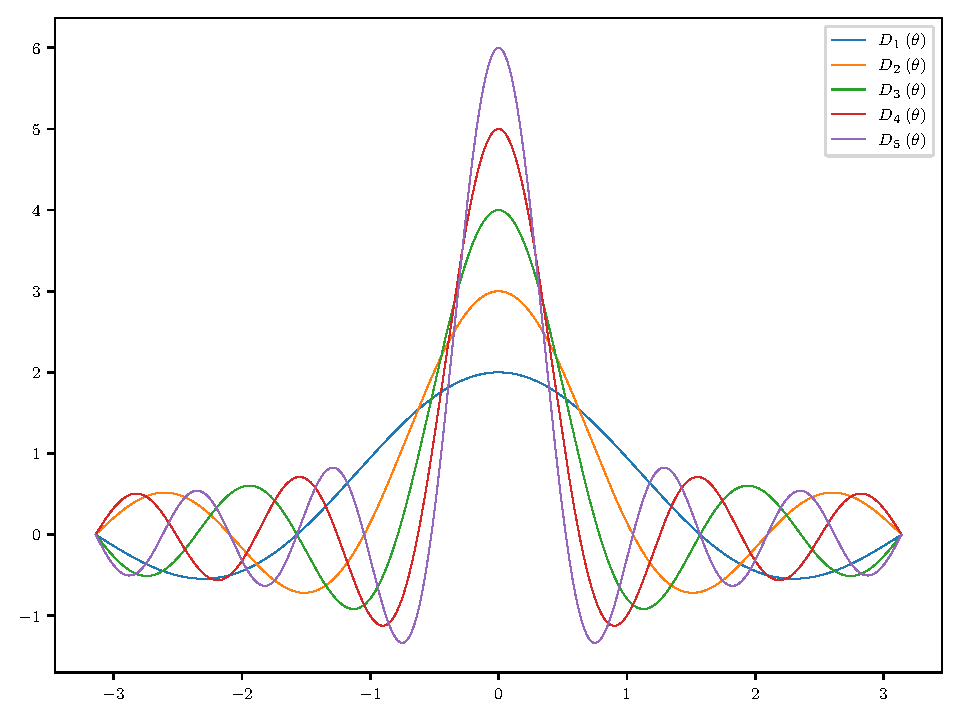
\includegraphics[width=0.35\paperwidth]{plot_dirichlet}
		\end{column}
		\begin{column}{0.54\textwidth}
			\begin{definition}[Dirichlet kernel]
				The \alert{Dirichlet kernel} $D_{n}$ of $n$-order is
				\begin{equation*}
					\fcolorbox{DarkBlue}{yellow}{
						\begin{math}
							\displaystyle
							D_{n}\left(\theta\right)\coloneqq
							\frac{1}{2}+
							\sum\limits_{k=1}^{n}\cos\left(k\theta\right)
						\end{math}
					}
				\end{equation*}
				$2\pi$-periodic and even, i.e.
				\begin{math}
					\forall\theta\in\mathds{R}:
					D\left(-\theta\right)=D\left(\theta\right)
				\end{math}.
			\end{definition}
		\end{column}
	\end{columns}

	\begin{definition}[Periodic function~\cite{Eisermann2023}]
		A function $f\colon\mathds{R}\to\mathds{C}$ is
		$T$-\alert{periodic} iff
		\begin{math}
			\exists T\in\mathds{R}\setminus\left\{0\right\}
		\end{math}
		such that
		\begin{math}
			\forall x\in\mathds{R}:
			f\left(x+T\right)=
			f\left(x\right)
		\end{math}.
	\end{definition}
	% https://math.stackexchange.com/a/3267091 % y par en $\left[0,T\right]$
	% \begin{theorem}[Integral $T$-periodic functions]% 1319p
	% 	The function $f\colon\mathds{R}\to\mathds{C}$ is
	% \end{theorem}
	\begin{block}{Remark}
		Let $x\in\mathds{R}$.
		If $f\in L\left(\left[0,T\right]\right)$ is $T$-periodic,
		then with the change of variable
		\begin{math}
			\alert{
				y\leftarrow\theta+x-\frac{T}{2}
			}
		\end{math}:

		\begin{equation*}
			\int\limits_{0}^{T}f\left(\theta\right)\dl\theta=
			\int\limits_{0}^{\frac{T}{2}}f\left(\theta\right)\dl\theta+
			\int\limits_{\frac{T}{2}}^{T}f\left(\theta\right)\dl\theta=
			\int\limits_{\alert{x-\frac{T}{2}}}^{\alert{x}}f\left(y\right)\dl y+
			\int\limits_{\alert{x}}^{\alert{x+\frac{T}{2}}}f\left(y\right)\dl y=
			\int\limits_{x-\frac{T}{2}}^{x+\frac{T}{2}}f\left(y\right)\dl y.
		\end{equation*}
	\end{block}
\end{frame}

\begin{frame}[allowframebreaks]
	%\frametitle{\secname}
	\begin{lemma}
		If $f\in L\left(\left[0,2\pi\right]\right)$ is $2\pi$-periodic,
		then the sequence of partial sum
		$\left\{s_{n}f\left(\theta\right)\right\}_{n\in\mathds{N}}$ of
		trigonometric Fourier series generated by $f$ has the integral
		representation
		\begin{equation*}
			\fcolorbox{DarkBlue}{yellow}{
				\begin{math}
					\displaystyle
					s_{n}f\left(\theta\right)=
					\frac{2}{\pi}\int\limits_{0}^{\pi}
					\frac{f\left(\theta+\xi\right)+f\left(\theta-\xi\right)}{2}
					D_{n}\left(\xi\right)\dl\xi.
				\end{math}
			}
		\end{equation*}
	\end{lemma}

	\begin{proof}
		\begin{align*}
			s_{n}f\left(\theta\right) & =
			\frac{\alert{a_{0}}}{2}+
			\sum_{k=1}^{n}
			\left(
			\alert{a_{k}}\cos\left(k\theta\right)+
			\alert{b_{k}}\sin\left(k\theta\right)
			\right).                      \\
			s_{n}f\left(\theta\right) & =
			\frac{1}{2}\cdot
			\alert{
				\frac{1}{\pi}
				\int\limits_{0}^{2\pi}
				f\left(\xi\right){\dl\xi}
			}+
			\sum_{k=1}^{n}
			\left(
			\alert{
				\frac{1}{\pi}
				\int\limits_{0}^{2\pi}
				f\left(\xi\right)\cos\left(k\xi\right){\dl\xi}
			}
			\cos\left(k\theta\right)+
			\alert{
				\frac{1}{\pi}
				\int\limits_{0}^{2\pi}
				f\left(\xi\right)\sin\left(k\xi\right){\dl\xi}
			}
			\sin\left(k\theta\right)
			\right).                      \\
			s_{n}f\left(\theta\right) & =
			\alert{
				\frac{1}{\pi}
				\int\limits_{0}^{2\pi}
				f\left(\xi\right)
			}
			\left(
			\frac{1}{2}
			+
			\sum_{k=1}^{n}
			\alert{\cos\left(k\xi\right)}
			\cos\left(k\theta\right)+
			\alert{\sin\left(k\xi\right)}
			\sin\left(k\theta\right)
			\right)
			\alert{{\dl\xi}}=
			\frac{1}{\pi}
			\int\limits_{0}^{2\pi}
			f\left(\xi\right)
			\left(
			\alert{
				\frac{1}{2}
				+
				\sum_{k=1}^{n}
				\cos\left(k\xi-k\theta\right)
			}
			\right)\dl\xi.
		\end{align*}

		\framebreak

		\begin{align*}
			s_{n}f\left(\theta\right) & =
			\frac{1}{\pi}
			\int\limits_{0}^{2\pi}
			f\left(\xi\right)
			\alert{
				D_{n}
				\left(
				k\left(\xi-\theta\right)
				\right)
			}
			\dl\xi.
			\shortintertext{
				The period of the product of two periodic functions $f$ and
				$D_{n}$ is the least common multiple of its periods, i.e.
				$\operatorname{lcm}\left(2\pi,2\pi\right)=2\pi$ and
				plugging the $u$-substitution $\alert{u=\xi-\theta}$.
			}
			s_{n}f\left(\theta\right) & =
			\frac{1}{\pi}
			\int\limits_{\theta-\pi}^{\theta+\pi}
			f\left(\alert{\xi}\right)
			D_{n}
			\left(
			k\left(\alert{\xi-\theta}\right)
			\right)
			\dl\xi=
			\frac{1}{\pi}
			\int\limits_{-\pi}^{\pi}
			f\left(\alert{\theta+u}\right)
			D_{n}
			\left(
			\alert{u}
			\right)
			\dl u.                        \\
			s_{n}f\left(\theta\right) & =
			\frac{1}{\pi}\left(
			\alert{\int\limits_{-\pi}^{0}}
			f\left(\theta+u\right)
			D_{n}
			\left(
			u
			\right)
			\dl u+
			\alert{\int\limits_{0}^{\pi}}
			f\left(\theta+u\right)
			D_{n}
			\left(
			u
			\right)
			\dl u
			\right).                      \\
			s_{n}f\left(\theta\right) & =
			\frac{1}{\pi}\left(
			\int\limits_{-\pi}^{0}
			f\left(\theta+u\right)
			\left(\alert{
				D_{n}
				\left(
				-u
				\right)
			}
			\right)
			\dl u+
			\int\limits_{0}^{\pi}
			f\left(\theta+u\right)
			D_{n}
			\left(
			u
			\right)
			\dl u
			\right).                      \\
			s_{n}f\left(\theta\right) & =
			\frac{1}{\pi}\left(
			\alert{\int\limits_{0}^{\pi}}
			f\left(\theta-u\right)
			D_{n}
			\left(
			u
			\right)
			\dl u+
			\alert{\int\limits_{0}^{\pi}}
			f\left(\theta+u\right)
			D_{n}
			\left(
			u
			\right)
			\dl u
			\right)=
			\frac{\alert{2}}{\pi}
			\alert{\int\limits_{0}^{\pi}}
			\frac{
				f\left(\theta+u\right)+
				f\left(\theta-u\right)
			}{\alert{2}}
			D_{n}
			\left(
			u
			\right)
			\dl u.
		\end{align*}
	\end{proof}
\end{frame}
\begin{frame}
	\frametitle{\secname}

	\begin{theorem}
		If $\theta\in\mathds{R}$, then
		\begin{equation*}
			\operatorname{Im}
			\left(
			\sum\limits_{k=1}^{n}
			e^{i\left(2k-1\right)\theta}
			\right)=
			\sum\limits_{k=1}^{n}
			\operatorname{Im}
			\left(
			e^{i\left(2k-1\right)\theta}
			\right)=
			\sum\limits_{k=1}^{n}
			\sin\left(\left(2k-1\right)\theta\right)=
			\begin{cases}
				\dfrac{\sin^{2}\left(n\theta\right)}{\sin\left(\theta\right)},
				 & \exists m\in\mathds{Z}
				\text{ such that }\theta\neq 2m\pi. \\
				0,
				 & \text{otherwise}.
			\end{cases}
		\end{equation*}
	\end{theorem}

	\begin{proof}
		Since
		\begin{math}
			\sum\limits_{k=1}^{n}
			{\left(e^{i\theta}\right)}^{k}=
			e^{i\left(n+1\right)\frac{\theta}{2}}
			\frac{
				\sin\left(n\frac{\theta}{2}\right)
			}{
				\sin\left(\frac{\theta}{2}\right)
			}
		\end{math}:

		\begin{align*}
			\sum\limits_{k=1}^{n}
			{
			\left(
			e^{i\theta}
			\right)
			}^{2k-1}
			        & =
			e^{-i\theta}
			\alert{
			\sum\limits_{k=1}^{n}
			{
			\left(
			e^{i2\theta}
			\right)
			}^{k}
			}=
			e^{-i\theta}
			\alert{e^{i\left(n+1\right)\theta}}
			\frac{
				\alert{\sin\left(n\theta\right)}
			}{
				\alert{\sin\left(\theta\right)}
			}=
			e^{in\theta}
			\frac{\sin\left(n\theta\right)}{\sin\left(\theta\right)}.
			\shortintertext{
				Taking the \alert{imaginary part} on the opposite sides of
				the equality:
			}
			\operatorname{Im}
			\left(
			\sum\limits_{k=1}^{n}
			e^{i\left(2k-1\right)\theta}
			\right) & =
			\sin\left(n\theta\right)
			\frac{\sin\left(n\theta\right)}{\sin\left(\theta\right)}=
			\frac{\sin^{2}\left(n\theta\right)}{\sin\left(\theta\right)}.
		\end{align*}
	\end{proof}
\end{frame}

\begin{frame}
	\frametitle{\secname}

	\begin{columns}
		\begin{column}{0.42\textwidth}
			\begin{figure}
				\centering
				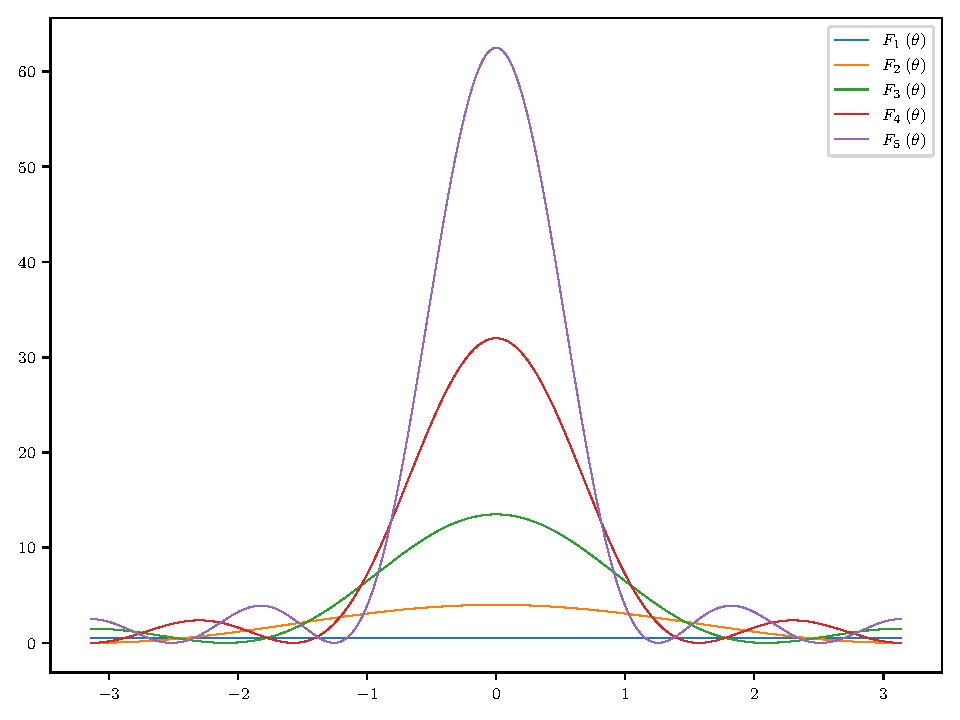
\includegraphics[width=0.35\paperwidth]{plot_fejer}
			\end{figure}
		\end{column}
		\begin{column}{0.54\textwidth}
			\begin{definition}[Fejér kernel]
				The \alert{Fejér kernel} $K_{n}$ of $n$-order is
				\begin{equation*}
					\fcolorbox{DarkBlue}{yellow}{
						\begin{math}
							\displaystyle
							K_{n}\left(\theta\right)\coloneqq
							\frac{1}{n}
							\sum_{k=1}^{n}D_{k-1}\left(\theta\right)
						\end{math}
					}
				\end{equation*}
				i.e. is the $n$-th Cesàro-Fourier means of the Dirichlet
				kernel.
			\end{definition}
		\end{column}
	\end{columns}

	\begin{definition}[$n$-th Cesàro-Fourier means]
		Let
		\begin{math}
			f\in L^{2}\left(\left[0,2\pi\right]\right)
		\end{math}.
		The \alert{$n$-th Cesàro-Fourier means} of $f$ is
		\begin{equation*}
			\fcolorbox{DarkBlue}{yellow}{
				\begin{math}
					\displaystyle
					\sigma_{n}f\left(\theta\right)=
					\frac{1}{n}\sum_{k=1}^{n}
					s_{k-1}f\left(\theta\right).
				\end{math}
			}
		\end{equation*}
	\end{definition}
\end{frame}

\begin{frame}
	\frametitle{\secname}

	\begin{lemma}
		If $f\in L\left(\left[0,2\pi\right]\right)$ is $2\pi$-periodic
		and $\left\{s_{n}f\left(\theta\right)\right\}_{n\in\mathds{N}}$
		is the sequence of partial sum of the trigonometric Fourier
		series generated by $f$.
		Then, the sequence
		\begin{math}
			\sigma_{n}
			f\left(\theta\right)
		\end{math}
		has the integral representation
		\begin{equation*}
			\fcolorbox{DarkBlue}{yellow}{
				\begin{math}
					\displaystyle
					\sigma_{n}f\left(\theta\right)=
					\frac{2}{\pi}
					\int\limits_{0}^{\pi}
					\frac{f\left(\theta+\xi\right)+f\left(\theta-\xi\right)}{2}
					K_{n}\left(\xi\right)\dl\xi.
				\end{math}
			}
		\end{equation*}
	\end{lemma}

	\begin{proof}
		If
		\begin{math}
			s_{n}f\left(\theta\right)=
			\displaystyle
			\frac{2}{\pi}
			\int\limits_{0}^{\pi}
			\frac{f\left(\theta+\xi\right)+f\left(\theta-\xi\right)}{2}
			D_{n}\left(\xi\right)\dl\xi
		\end{math},
		then
		\begin{align*}
			\sigma_{n}f\left(\theta\right)
			 & =
			\dfrac{1}{n}
			\sum\limits_{k=1}^{n}
			\alert{s_{k-1}f\left(\theta\right)}
			= \frac{1}{n}
			\sum\limits_{k=1}^{n}
			\alert{
				\frac{2}{\pi}
				\int\limits_{0}^{\pi}
				\frac{f\left(\theta+\xi\right)+f\left(\theta-\xi\right)}{2}
				D_{k-1}\left(\xi\right){\dl\xi}
			}.   \\
			\sigma_{n}f\left(\theta\right)
			 & =
			\frac{2}{\pi}
			\int\limits_{0}^{\pi}
			\frac{f\left(\theta+\xi\right)+f\left(\theta-\xi\right)}{2}
			\alert{
				\frac{1}{n}\sum\limits_{k=1}^{n}
				D_{k-1}\left(\xi\right)
			}
			\dl\xi
			=
			\frac{2}{\pi}
			\int\limits_{0}^{\pi}
			\frac{f\left(\theta+\xi\right)+f\left(\theta-\xi\right)}{2}
			\alert{K_{n}\left(\xi\right)}
			\dl\xi.
		\end{align*}
	\end{proof}
\end{frame}

\begin{frame}[allowframebreaks]
	% \frametitle{\secname}

	\begin{theorem}
		Let $\theta\in\mathds{R}$.
		$\forall n\in\mathds{N}$:

		\begin{columns}
			\begin{column}{0.38\textwidth}
				\begin{itemize}
					\item

					      \begin{math}
						      \displaystyle
						      \int\limits_{0}^{\pi}
						      K_{n}\left(\theta\right)=
						      \frac{\pi}{2}
					      \end{math}.

					\item

					      \begin{math}
						      \displaystyle
						      K_{n}\left(\theta\right)=
						      \dfrac{1}{2n}
						      \dfrac{
							      \sin^{2}\left(n\dfrac{\theta}{2}\right)
						      }{
							      \sin^{2}\left(\dfrac{\theta}{2}\right)
						      }
						      \geq0
					      \end{math}.
				\end{itemize}
			\end{column}
			\begin{column}{0.58\textwidth}
				\begin{itemize}
					\item

					      \begin{math}
						      \displaystyle
						      \forall\delta\in\left(0,\pi\right):
						      \forall\delta\leq\left|\theta\right|\leq\pi:
						      K_{n}\left(\theta\right)
						      \leq
						      \frac{1}{
							      2n\sin^{2}\left(\frac{\delta}{2}\right)
						      }
					      \end{math}.
				\end{itemize}
			\end{column}
		\end{columns}
	\end{theorem}

	\begin{proof}
		\begin{itemize}
			\item

			      \begin{align*}
				      K_{n}\left(\theta\right) & =
				      \frac{1}{n}
				      \sum_{k=1}^{n}
				      \alert{D_{k-1}\left(\theta\right)}=
				      \frac{1}{n}
				      \sum_{k=1}^{n}
				      \left(
				      \alert{
					      \frac{1}{2}+
					      \sum_{m=1}^{k-1}
					      \cos\left(m\theta\right)
				      }
				      \right)=
				      \frac{1}{n}
				      \left(
				      \sum_{k=1}^{n}
				      \alert{\frac{1}{2}}+
				      \sum_{k=1}^{n}
				      \alert{
					      \sum_{m=1}^{k-1}
					      \cos\left(m\theta\right)
				      }
				      \right).                     \\
				      \int\limits_{0}^{\pi}
				      K_{n}\left(\theta\right)
				                               & =
				      \int\limits_{0}^{\pi}
				      \frac{1}{n}
				      \left(
				      \alert{\sum_{k=1}^{n}}
				      \frac{\alert{1}}{2}+
				      \sum_{k=1}^{n}
				      \sum_{m=1}^{k-1}
				      \cos\left(m\theta\right)
				      \right)
				      \dl\theta
				      =
				      \frac{1}{n}
				      \left(
				      \frac{\alert{n}}{2}
				      \alert{
					      \int\limits_{0}^{\pi}
					      {\dl\theta}
				      }
				      +
				      \sum_{k=1}^{n}
				      \sum_{m=1}^{k-1}
				      \alert{
					      \int\limits_{0}^{\pi}
					      \cos\left(m\theta\right)
					      {\dl\theta}
				      }
				      \right)
				      =
				      \frac{1}{n}
				      \left(
				      \frac{n\alert{\pi}}{2}+\alert{0}
				      \right)=
				      \frac{\pi}{2}.
			      \end{align*}
		\end{itemize}

		\framebreak

		\begin{itemize}
			\item

			      \begin{align*}
				      K_{n}\left(\theta\right) & =
				      \frac{1}{n}
				      \left(
				      \alert{
					      \sum_{k=1}^{n}
				      }
				      \frac{\alert{1}}{2}+
				      \sum_{k=1}^{n}
				      \alert{
					      \sum_{m=1}^{k-1}
					      \cos\left(m\theta\right)
				      }
				      \right)
				      =
				      \frac{1}{n}
				      \left(
				      \frac{\alert{n}}{2}+
				      \sum_{k=1}^{n}
				      \left(
					      \alert{
						      \frac{
							      \sin
							      \left(
							      \left(2\left(k-1\right)+1\right)
							      \frac{\theta}{2}
							      \right)
						      }{
							      2\sin\left(\frac{\theta}{2}\right)
						      }-\frac{1}{2}
					      }
					      \right)
				      \right)                      \\
				      K_{n}\left(\theta\right) & =
				      \frac{1}{n}
				      \left(
				      \frac{n}{2}+
				      \frac{
						      \sum\limits_{k=1}^{n}
						      \sin
						      \left(
						      \left(2\left(k-1\right)+1\right)
						      \frac{\theta}{2}
						      \right)
					      }{
						      2\sin\left(\frac{\theta}{2}\right)
					      }-
				      \alert{
						      \sum_{k=1}^{n}
					      }
				      \frac{\alert{1}}{2}
				      \right)
				      =
				      \frac{1}{n}
				      \left(
				      \frac{n}{2}+
				      \frac{
					      \alert{
						      \sum\limits_{k=1}^{n}
						      \sin\left(\left(2k-1\right)\frac{\theta}{2}\right)
					      }
				      }{
					      2\sin\left(\frac{\theta}{2}\right)
				      }
				      -\frac{\alert{n}}{2}
				      \right)                      \\
				      K_{n}\left(\theta\right) & =
				      \frac{1}{2n}
				      \frac{
					      \alert{
						      \frac{
							      \sin^{2}\left(n\frac{\theta}{2}\right)
						      }{
							      \sin\left(\frac{\theta}{2}\right)
						      }
					      }
				      }{\sin\left(\frac{\theta}{2}\right)}=
				      \frac{1}{2n}
				      \frac{
					      \sin^{2}\left(n\frac{\theta}{2}\right)
				      }{
					      \sin^{2}\left(\frac{\theta}{2}\right)
				      }
				      \geq0.
			      \end{align*}

			\item

			      \begin{math}
				      \forall\delta\in\left(0,\pi\right):
				      \sin^{2}\left(\frac{\delta}{2}\right)
			      \end{math}
			      is \alert{even} and increasing.
			      Then,
			      \begin{math}
				      \forall
				      \delta<
				      \left|\theta\right|
				      <\pi
			      \end{math}:

			      \begin{equation*}
				      \frac{\delta}{2}<
				      \frac{\left|\theta\right|}{2}
				      \implies
				      \sin^{2}\left(\frac{\delta}{2}\right)<
				      \alert{
					      \sin^{2}\left(\frac{\left|\theta\right|}{2}\right)
				      }
				      \implies
				      \sin^{2}\left(\frac{\delta}{2}\right)
				      <
				      \alert{\sin^{2}\left(\frac{\theta}{2}\right)}
				      \implies
				      \frac{1}{\sin^{2}\left(\frac{\theta}{2}\right)}<
				      \frac{1}{\sin^{2}\left(\frac{\delta}{2}\right)}.
			      \end{equation*}

			      \begin{align*}
				      K_{n}\left(\theta\right)
				      =
				      \frac{1}{2n}
				      \frac{
					      \sin^{2}\left(n\frac{\theta}{2}\right)
				      }{
					      \sin^{2}\left(\frac{\theta}{2}\right)
				      }
				      =
				      \frac{
					      \alert{
						      \sin^{2}\left(n\frac{\theta}{2}\right)
					      }
				      }{
					      2n
					      \alert{
						      \sin^{2}\left(\frac{\theta}{2}\right)
					      }
				      }\leq
				      \frac{\alert{1}}{
					      2n
					      \alert{
						      \sin^{2}\left(\frac{\delta}{2}\right)
					      }
				      }.
			      \end{align*}
		\end{itemize}
	\end{proof}
\end{frame}

\begin{frame}
	\frametitle{\secname}

	\begin{block}{Remark}
		Applying the last lemma for
		\begin{math}
			\alert{f\equiv 1}\in
			L\left(\left[0,2\pi\right]\right)
		\end{math}
		which is $2\pi$-periodic, then
		\begin{math}
			\forall n\in\mathds{N}
		\end{math}:
		\begin{align*}
			s_{n}f\left(\theta\right)      & =
			\frac{2}{\pi}
			\int\limits_{0}^{\pi}
			\frac{f\left(\theta+\xi\right)+f\left(\theta-\xi\right)}{2}
			\alert{D_{n}\left(\xi\right)}
			\dl\xi
			=
			\frac{2}{\pi}
			\int\limits_{0}^{\pi}
			\frac{\alert{1}+\alert{1}}{2}
			\left(
			\alert{\frac{1}{2}+\sum_{k=1}^{n}\cos\left(k\xi\right)}
			\right)
			\dl\xi
			=
			\frac{2}{\pi}
			\int\limits_{0}^{\pi}
			\left(
			\frac{1}{2}+\sum_{k=1}^{n}\cos\left(k\xi\right)
			\right)
			\dl\xi                             \\
			s_{n}f\left(\theta\right)      & =
			\frac{2}{\pi}
			\int\limits_{0}^{\pi}
			\frac{\dl\xi}{2}
			+
			\frac{2}{\pi}
			\int\limits_{0}^{\pi}
			\sum_{k=1}^{n}
			\cos\left(k\xi\right)
			\dl\xi
			=
			1+
			\frac{2}{\pi}
			\sum_{k=1}^{n}
			\alert{
				\int\limits_{0}^{\pi}
				\cos\left(k\xi\right)
				{\dl\xi}
			}
			=
			1+
			\frac{2}{\pi}
			\sum_{k=1}^{n}
			\alert{
				{
						\left(
						\frac{\sin\left(k\xi\right)}{k}
						\right)
						\Biggr|
					}_{0}^{\pi}
			}
			=
			1+
			\frac{2}{\pi}
			\sum_{k=1}^{n}
			\alert{0}=
			1.                                 \\
			\sigma_{n}f\left(\theta\right) & =
			\frac{2}{\pi}
			\int\limits_{0}^{\pi}
			\frac{f\left(\theta+\xi\right)+f\left(\theta-\xi\right)}{2}
			K_{n}\left(\xi\right)
			\dl\xi=
			\frac{2}{\pi}
			\int\limits_{0}^{\pi}
			\frac{\alert{1}+\alert{1}}{2}
			K_{n}\left(\xi\right)
			\dl\xi
			=
			\frac{2}{\pi}
			\alert{
				\int\limits_{0}^{\pi}
				K_{n}\left(\xi\right)
				{\dl\xi}
			}
			=
			\frac{2}{\pi}\cdot
			\alert{\frac{\pi}{2}}
			=
			1.
		\end{align*}
		We will see if
		\begin{math}
			sf\left(\theta\right)\coloneqq
			\lim\limits_{\xi\to0^{+}}
			\dfrac{
				f\left(\theta+\xi\right)+f\left(\theta-\xi\right)
			}{2}\in\mathds{R}
		\end{math},
		then
		\begin{math}
			{
				\left\{
				\sigma_{n}f\left(\theta\right)-
				sf\left(\theta\right)
				\right\}
			}_{n\in\mathds{N}}
		\end{math}
		converges to $0\in L\left(\left[0,2\pi\right]\right)$.
		\begin{gather}
			\sigma_{n}f\left(\theta\right)-
			sf\left(\theta\right)\cdot\alert{1}=
			\frac{2}{\pi}
			\int\limits_{0}^{\pi}
			\frac{
				f\left(\theta+\xi\right)+
				f\left(\theta-\xi\right)
			}{2}
			K_{n}\left(\xi\right)
			\dl\xi
			-
			sf\left(\theta\right)
			\alert{
				\frac{2}{\pi}
				\int_{0}^{\pi}
				K_{n}\left(\xi\right)
				{\dl\xi}
			}.\notag                                \\
			\fcolorbox{DarkBlue}{yellow}{
				\begin{math}
					\displaystyle
					\sigma_{n}f\left(\theta\right)-
					sf\left(\theta\right)
					=
					\frac{2}{\pi}
					\int\limits_{0}^{\pi}
					\left(
					\frac{
							f\left(\theta+\xi\right)+
							f\left(\theta-\xi\right)
						}{2}-sf\left(\theta\right)
					\right)
					K_{n}\left(\xi\right)
					\dl\xi.
				\end{math}
			}\label{eq:mean-difference}\tag{$\bigstar$}
		\end{gather}
	\end{block}
\end{frame}
\section{Fejér's theorem}
% Fejér, L., 82, 139, 142, 152, 153, 728
\begin{frame}[allowframebreaks]
	% \frametitle{\secname}
	% https://en.wikipedia.org/wiki/Fej%C3%A9r%27s_theorem
	% una función integrable de Lebesgue y que es 
	\begin{theorem}[\secname]
		If $f\in L\left(\left[0,2\pi\right]\right)$ is $2\pi$-periodic
		and $sf\left(\theta\right)\in\mathds{R}$, then
		\begin{math}
			\forall\theta\in\operatorname{dom}\left(sf\right):
			\left\{
			\sigma_{n}f\left(\theta\right)
			\right\}_{n\in\mathds{N}}
		\end{math}
		is Cesàro summable.
		I.e.
		\begin{equation*}
			\lim\limits_{n\to\infty}
			\sigma_{n}f\left(\theta\right)=
			\lim\limits_{n\to\infty}
			\frac{1}{n}\sum_{k=1}^{n}s_{n}f\left(\theta\right)=
			sf\left(\theta\right).
		\end{equation*}

		If $f$ is continuous on $\left[0,2\pi\right]$, then
		\begin{math}
			\left\{
			\sigma_{n}f
			\right\}_{n\in\mathds{N}}
		\end{math}
		converges uniformily
		to $f$ on $\left[0,2\pi\right]$.
	\end{theorem}

	\begin{proof}
		Suppose that $f\in L\left(\left[0,2\pi\right]\right)$ is
		$2\pi$-periodic and $\theta\in\operatorname{dom}\left(sf\right)$.
		We define
		\begin{align*}
			g_{\theta}\colon\left[0,2\pi\right]
			 & \to\mathds{R} \\
			\xi
			 & \mapsto
			\frac{
				f\left(\theta+\xi\right)+f\left(\theta-\xi\right)
			}{2}-sf\left(\theta\right).
		\end{align*}
		Then,
		\begin{equation*}
			\lim\limits_{\xi\to0^{+}}
			\alert{g_{\theta}\left(\xi\right)}=
			\lim\limits_{\xi\to0^{+}}
			\left(
			\alert{
				\dfrac{
					f\left(\theta+\xi\right)+f\left(\theta-\xi\right)
				}{2}-
				sf\left(\theta\right)
			}
			\right)=
			\alert{
				\lim\limits_{\xi\to0^{+}}
				\dfrac{
					f\left(\theta+\xi\right)+f\left(\theta-\xi\right)
				}{2}
			}
			-sf\left(\theta\right)=
			\alert{sf\left(\theta\right)}-
			sf\left(\theta\right)
			=
			0.
		\end{equation*}
		I.e.
		\begin{math}
			\forall\varepsilon>0:
			\exists
			0<\delta_{\xi}<\pi
		\end{math}
		such that
		\begin{math}
			\forall 0<\xi<\delta_{\xi}:
			\fcolorbox{DarkBlue}{yellow}{
				\begin{math}
					\left|g_{\theta}\left(\xi\right)\right|<
					\dfrac{\varepsilon}{2}
				\end{math}
			}
		\end{math}.

		\framebreak

		\begin{itemize}
			\item

			      Let $n\in\mathds{N}$ and $\xi\in\left[0,\delta\right]$.
		\end{itemize}

		\begin{align*}
			\left|
			\sigma_{n}f
			\left(\theta\right)-sf\left(\theta\right)
			\right|
			 & =
			\left|
			\frac{2}{\pi}
			\int\limits_{0}^{\delta}
			\left(
			\alert{
				\frac{
					f\left(\theta+\xi\right)+
					f\left(\theta-\xi\right)
				}{2}-sf\left(\theta\right)
			}
			\right)
			K_{n}\left(\xi\right)
			\dl\xi
			\right|
			=
			\left|
			\frac{2}{\pi}
			\int\limits_{0}^{\delta}
			\alert{
				g_{\theta}\left(\xi\right)
			}
			K_{n}\left(\xi\right)
			\dl\xi
			\right|
			\leq
			\frac{2}{\pi}
			\int\limits_{0}^{\delta}
			\alert{
				\left|
				g_{\theta}\left(\xi\right)
				\right|
			}
			\left|
			K_{n}\left(\xi\right)
			\right|
			\dl\xi. \\
			\left|
			\sigma_{n}f
			\left(\theta\right)-sf\left(\theta\right)
			\right|
			 & <
			\frac{2}{\pi}
			\int\limits_{0}^{\delta}
			\alert{\frac{\varepsilon}{2}}
			\left|
			K_{n}\left(\xi\right)
			\right|
			\dl\xi
			=
			\frac{\varepsilon}{\pi}
			\alert{\int\limits_{0}^{\delta}}
			K_{n}\left(\xi\right)
			\dl\xi
			<
			\frac{\varepsilon}{\pi}
			\alert{\int\limits_{0}^{\pi}}
			K_{n}\left(\xi\right)
			\dl\xi
			=
			\frac{\varepsilon}{\pi}\cdot
			\alert{\frac{\pi}{2}}=
			\frac{\varepsilon}{2}.
		\end{align*}

		\begin{itemize}
			\item

			      Let $n\in\mathds{N}$ and $\xi\in\left[\delta,\pi\right]$.
			      Since
			      \begin{math}
				      g_{\theta}\in
				      L\left(\left[0,2\pi\right]\right),
			      \end{math}
			      then
			      \begin{math}
				      \displaystyle
				      M=
				      \alert{
					      \int\limits_{\delta}^{\pi}
				      }
				      \left|g_{\theta}\left(\xi\right)\right|
				      \dl\xi
				      \leq
				      \alert{
					      \int\limits_{0}^{2\pi}
				      }
				      \left|g_{\theta}\left(\xi\right)\right|
				      \dl\xi
				      <\infty
			      \end{math}.
		\end{itemize}

		\begin{align*}
			\left|
			\sigma_{n}f\left(\theta\right)-
			sf\left(\theta\right)
			\right| & \leq
			\frac{2}{\pi}
			\int\limits_{\delta}^{\pi}
			\left|
			g_{\theta}\left(\xi\right)
			\right|
			\alert{
				\left|
				K_{n}\left(\xi\right)
				\right|
			}
			\dl\xi=
			\frac{2}{\pi}
			\int\limits_{\delta}^{\pi}
			\left|
			g_{\theta}\left(\xi\right)
			\right|
			\alert{K_{n}\left(\xi\right)}
			\dl\xi
			\leq
			\frac{2}{\pi}
			\int\limits_{\delta}^{\pi}
			\left|
			g_{\theta}\left(\xi\right)
			\right|
			\alert{
				\frac{1}{
					2n\sin^{2}\left(\frac{\delta}{2}\right)
				}
			}
			\dl\xi
			=
			\int\limits_{\delta}^{\pi}
			\frac{
				\left|
				g_{\theta}\left(\xi\right)
				\right|
			}{
				n\pi\sin^{2}\left(\frac{\delta}{2}\right)
			}
			\dl\xi.
		\end{align*}
		Since $\mathds{R}$ is an \alert{archimedean} ordered field,
		satisfies the \alert{archimedean property}, i.e.

		\begin{equation*}
			\forall\varepsilon>0:
			\forall L\in\mathds{R}:
			\exists n_{0}\in\mathds{N}
			\text{ such that }
			\frac{1}{n_{0}}L<
			\frac{\varepsilon}{2}.
		\end{equation*}
	\end{proof}
\end{frame}

\begin{frame}
	\begin{proof}
		Let
		\begin{math}
			L=
			\dfrac{
				\alert{M}
			}{
				\pi\sin^{2}\left(\frac{\delta}{2}\right)
			}
		\end{math}.
		Next,
		\begin{math}
			\displaystyle
			\forall\varepsilon>0:
			\forall L\in\mathds{R}:
			\exists n_{0}\in\mathds{N}
			\text{ such that }
			\frac{1}{n_{0}}
			\frac{
			\alert{
			\int\limits_{\delta}^{\pi}
			\left|g_{\theta}\left(\xi\right)\right|
			\dl\xi}
			}{\pi\sin^{2}\left(\frac{\delta}{2}\right)}
			<\frac{\varepsilon}{2}
		\end{math}.
		Then, $\forall n>n_{0}$:

		\begin{align*}
			\frac{1}{n}                                 & <
			\frac{1}{n_{0}}.                                \\
			\alert{\frac{1}{n}}
			\frac{
				\left|
				g_{\theta}\left(\xi\right)
				\right|
			}{\pi\sin^{2}\left(\frac{\delta}{2}\right)} & <
			\alert{\frac{1}{n_{0}}}
			\frac{
				\left|
				g_{\theta}\left(\xi\right)
				\right|
			}{\pi\sin^{2}\left(\frac{\delta}{2}\right)}.    \\
			\left|
			\sigma_{n}f\left(\theta\right)-
			sf\left(\theta\right)
			\right|\leq
			\alert{
				\int\limits_{\delta}^{\pi}
				\frac{1}{n}
			}
			\frac{
				\left|
				g_{\theta}\left(\xi\right)
				\right|
			}{
				\pi\sin^{2}\left(\frac{\delta}{2}\right)
			}
			\dl\xi
			                                            & <
			\alert{
				\int\limits_{\delta}^{\pi}
				\frac{1}{n_{0}}
			}
			\frac{
			\left|g_{\theta}\left(\xi\right)\right|
			}{\pi\sin^{2}\left(\frac{\delta}{2}\right)}
			\dl\xi=
			\frac{1}{n_{0}}
			\frac{
			\int\limits_{\delta}^{\pi}
			\left|g_{\theta}\left(\xi\right)\right|
			\dl\xi
			}{\pi\sin^{2}\left(\frac{\delta}{2}\right)}
			<\frac{\varepsilon}{2}.
		\end{align*}

		I.e.
		\begin{math}
			\forall\varepsilon>0:
			\exists n_{0}\in\mathds{N}
			\text{ such that }
			\forall n\geq n_{0}:
		\end{math}

		\begin{equation*}
			\left|
			\sigma_{n}f\left(\theta\right)-
			sf\left(\theta\right)
			\right|
			\leq
			\frac{2}{\pi}
			\alert{\int\limits_{0}^{\pi}}
			\left|
			g_{\theta}\left(\xi\right)
			\right|
			K_{n}\left(\xi\right)
			\dl\xi
			=
			\frac{2}{\pi}
			\alert{\int\limits_{0}^{\delta}}
			\left|
			g_{\theta}\left(\xi\right)
			\right|
			K_{n}\left(\xi\right)
			\dl\xi
			+
			\frac{2}{\pi}
			\alert{\int\limits_{\delta}^{\pi}}
			\left|
			g_{\theta}\left(\xi\right)
			\right|
			K_{n}\left(\xi\right)
			\dl\xi
			<\frac{\varepsilon}{2}+
			\frac{\varepsilon}{2}=
			\varepsilon.
		\end{equation*}
	\end{proof}
\end{frame}

\begin{frame}[allowframebreaks]
	\begin{proof}
		Suppose that $f$ is continuous in $\left[0,2\pi\right]$.
		We define
		\begin{align*}
			h_{\theta}\colon\left[0,2\pi\right]
			 & \to\mathds{R} \\
			\xi
			 & \mapsto
			\frac{
				f\left(\theta+\xi\right)+f\left(\theta-\xi\right)
			}{2}-f\left(\theta\right).
		\end{align*}
		Since $f$ is continuous in $\left[0,2\pi\right]$, $h_{\theta}$ is
		uniformily continuous in $\left[0,2\pi\right]$.
		I.e.
		\begin{math}
			\forall\varepsilon>0:
			\exists
			0<\delta<\pi
		\end{math}
		such that
		\begin{math}
			\forall\xi_{1},\xi_{2}\in\left[0,2\pi\right]
		\end{math}:

		\begin{equation*}
			\left|
			\xi_{1}-\xi_{2}
			\right|<\delta
			\implies
			\left|
			h_{\theta}\left(\xi_{1}\right)-
			h_{\theta}\left(\xi_{2}\right)
			\right|<
			\dfrac{\varepsilon}{2}.
		\end{equation*}

		Hence, for $\xi_{1}=\xi$ and $\xi_{2}=0$:
		\begin{math}
			\left|
			h_{\theta}\left(\xi\right)-
			\alert{h_{\theta}\left(0\right)}
			\right|
			=
			\left|
			h_{\theta}\left(\xi\right)-
			\alert{
				\left(
				\frac{f\left(\theta+0\right)+f\left(\theta-0\right)}{2}-
				f\left(\theta\right)
				\right)
			}
			\right|
			=
			\fcolorbox{DarkBlue}{yellow}{
				\begin{math}
					\left|
					h_{\theta}\left(\xi\right)
					\right|
					<
					\dfrac{\varepsilon}{2}
				\end{math}
			}
		\end{math}.

		In other hand,
		\begin{align*}
			\left|
			\alert{\sigma_{n}f\left(\theta\right)}-
			f\left(\theta\right)\cdot\alert{1}
			\right| & =
			\left|
			\alert{
				\frac{2}{\pi}
				\int\limits_{0}^{\pi}
				\frac{f\left(\theta+\xi\right)+f\left(\theta-\xi\right)}{2}
				K_{n}\left(\xi\right)\dl\xi
			}
			-
			f\left(\theta\right)
			\alert{
				\frac{2}{\pi}
				\int_{0}^{\pi}
				K_{n}\left(\xi\right)
				\dl\xi
			}
			\right|=
			\left|
			\frac{2}{\pi}
			\int\limits_{0}^{\pi}
			h_{\theta}\left(\xi\right)
			K_{n}\left(\xi\right)\dl\xi
			\right|        \\
			        & \leq
			\frac{2}{\pi}
			\int\limits_{0}^{\pi}
			\left|
			h_{\theta}\left(\xi\right)
			\right|
			\left|
			K_{n}\left(\xi\right)
			\right|
			\dl\xi=
			\frac{2}{\pi}
			\int\limits_{0}^{\pi}
			\left|
			h_{\theta}\left(\xi\right)
			\right|
			K_{n}\left(\xi\right)
			\dl\xi.
		\end{align*}

		\framebreak

		\begin{itemize}
			\item

			      Let $n\in\mathds{N}$ and $\xi\in\left[0,\delta\right]$.

		\end{itemize}

		\begin{equation*}
			\left|
			\sigma_{n}f\left(\theta\right)-
			f\left(\theta\right)
			\right|
			\leq
			\frac{2}{\pi}
			\int\limits_{0}^{\delta}
			\alert{
				\left|
				h_{\theta}\left(\xi\right)
				\right|
			}
			K_{n}\left(\xi\right)
			\dl\xi
			<
			\frac{2}{\pi}
			\int\limits_{0}^{\delta}
			\alert{
				\frac{\varepsilon}{2}
			}
			K_{n}\left(\xi\right)
			\dl\xi
			<
			\frac{\varepsilon}{\pi}
			\alert{
				\int\limits_{0}^{\pi}
				K_{n}\left(\xi\right)
				\dl\xi
			}
			=\frac{\varepsilon}{\pi}\cdot
			\alert{\frac{\pi}{2}}=
			\frac{\varepsilon}{2}.
		\end{equation*}

		\begin{itemize}
			\item

			      Let $n\in\mathds{N}$ and $\xi\in\left[\delta,\pi\right]$.
			      Since $h_{\theta}$ is bounded on
			      $\left[\delta,\pi\right]$, attains the maximum
			      \begin{math}
				      \alert{M}
				      \coloneqq
				      \max\limits_{\theta\in\left[\delta,\pi\right]}
				      \left|
				      h_{\theta}
				      \right|
			      \end{math}.
		\end{itemize}

		\begin{equation*}
			\left|
			\sigma_{n}f\left(\theta\right)-
			f\left(\theta\right)
			\right|
			\leq
			\frac{2}{\pi}
			\int\limits_{\delta}^{\pi}
			\alert{
				\left|
				h_{\theta}\left(\xi\right)
				\right|
			}
			K_{n}\left(\xi\right)
			\dl\xi
			\leq
			\frac{2}{\pi}
			\int\limits_{\delta}^{\pi}
			\alert{M}
			K_{n}\left(\xi\right)
			\dl\xi
			\leq
			\frac{2}{\pi}
			\int\limits_{\delta}^{\pi}
			\alert{
				\frac{M}{
					2n\sin^{2}\left(\frac{\delta}{2}\right)
				}
			}
			\dl\xi=
			\int\limits_{\delta}^{\pi}
			\frac{M}{n\pi\sin^{2}\left(\frac{\delta}{2}\right)}
			\dl\xi.
		\end{equation*}

		Since $\mathds{R}$ is an \alert{archimedean} ordered field,
		satisfies the \alert{archimedean property}, i.e.

		\begin{equation*}
			\forall\varepsilon>0:
			\forall L\in\mathds{R}:
			\exists n_{0}\in\mathds{N}
			\text{ such that }
			\frac{1}{n_{0}}L<
			\frac{\varepsilon}{2}.
		\end{equation*}

		Let
		\begin{math}
			L=
			\dfrac{
				M
			}{
				\pi\sin^{2}\left(\frac{\delta}{2}\right)
			}
		\end{math}.
		Next,
		\begin{math}
			\displaystyle
			\forall\varepsilon>0:
			\forall L\in\mathds{R}:
			\exists n_{0}\in\mathds{N}
			\text{ such that }
			\frac{1}{n_{0}}
			\frac{
				M
			}{\pi\sin^{2}\left(\frac{\delta}{2}\right)}
			<\frac{\varepsilon}{2}
		\end{math}.
		Then, $\forall n>n_{0}$:

		\framebreak

		\begin{align*}
			\frac{1}{n}                                 & <
			\frac{1}{n_{0}}.                                \\
			\alert{\frac{1}{n}}
			\frac{
				M
			}{\pi\sin^{2}\left(\frac{\delta}{2}\right)} & <
			\alert{\frac{1}{n_{0}}}
			\frac{
				M
			}{\pi\sin^{2}\left(\frac{\delta}{2}\right)}.    \\
			\left|
			\sigma_{n}f\left(\theta\right)-
			f\left(\theta\right)
			\right|\leq
			\alert{
				\int\limits_{\delta}^{\pi}
				\frac{1}{n}
			}
			\frac{
				M
			}{
				\pi\sin^{2}\left(\frac{\delta}{2}\right)
			}
			\dl\xi
			                                            & <
			\alert{
				\int\limits_{\delta}^{\pi}
				\frac{1}{n_{0}}
			}
			\frac{
				M
			}{\pi\sin^{2}\left(\frac{\delta}{2}\right)}
			\dl\xi=
			\frac{1}{n_{0}}
			\frac{
				M
			}{\pi\sin^{2}\left(\frac{\delta}{2}\right)}
			<\frac{\varepsilon}{2}.
		\end{align*}

		I.e.
		\begin{math}
			\forall\varepsilon>0:
			\exists n_{0}\in\mathds{N}
			\text{ such that }
			\forall n\geq n_{0}:
			\forall\theta\in\left[0,2\pi\right]:
		\end{math}

		\begin{equation*}
			\left|
			\sigma_{n}f\left(\theta\right)-
			f\left(\theta\right)
			\right|
			\leq
			\frac{2}{\pi}
			\alert{\int\limits_{0}^{\pi}}
			\left|
			h_{\theta}\left(\xi\right)
			\right|
			K_{n}\left(\xi\right)
			\dl\xi
			=
			\frac{2}{\pi}
			\alert{\int\limits_{0}^{\delta}}
			\left|
			h_{\theta}\left(\xi\right)
			\right|
			K_{n}\left(\xi\right)
			\dl\xi
			+
			\frac{2}{\pi}
			\alert{\int\limits_{\delta}^{\pi}}
			\left|
			h_{\theta}\left(\xi\right)
			\right|
			K_{n}\left(\xi\right)
			\dl\xi
			<\frac{\varepsilon}{2}+
			\frac{\varepsilon}{2}=
			\varepsilon.
		\end{equation*}
	\end{proof}
\end{frame}
\section{Weierstraß approximation theorem}

\begin{frame}
	Let is remember from the course of Complex analysis.

	\begin{definition}[Power series]
		An infinite series
		\begin{equation*}
			a_{0}+
			\sum_{n=1}^{\infty}
			a_{n}
				{\left(z-z_{0}\right)}^{n}
		\end{equation*}
		is a \alert{power series} in $z-z_{0}$.
	\end{definition}

	\begin{theorem}
		Let
		\begin{math}
			a_{0}+
			\sum\limits_{n=1}^{\infty}
			a_{n}
				{\left(z-z_{0}\right)}^{n}
		\end{math}
		be a power series.
		\begin{equation*}
			\frac{1}{R}=
			\limsup_{n\to\infty}\sqrt[n]{\left|a_{n}\right|}.
		\end{equation*}
		Then, the series converges absolutely if
		\begin{math}
			\left|z-z_{0}\right|<R
		\end{math}
		and diverges if
		\begin{math}
			\left|z-z_{0}\right|>R
		\end{math}.
		Also, the series converges uniformily on every compact subset
		interior to the disk of convergence.
	\end{theorem}

	\begin{definition}[Power series expansion]
		The \alert{power series expansion} of a function $f$ about a
		given point $z_{0}$ is uniquely determined by
		\begin{equation*}
			f\left(z\right)=
			\sum_{n=0}^{\infty}
			\frac{f^{\left(n\right)}\left(z_{0}\right)}{n!}
			{\left(z-z_{0}\right)}^{n}.
		\end{equation*}
	\end{definition}
\end{frame}

% \begin{frame}
% 	\begin{theorem}[Abel limit theorem]
% 		Suppose that the complex power series
% 		\begin{math}
% 			\sum\limits_{n=0}^{\infty}
% 			a_{n}x^{n}
% 		\end{math}
% 		converge absolutamente en un punto $x_{0}$,
% 		entonces la serie de potencias converge uniformemente en
% 		un intervalo compacto $\left[-c,c\right]$, donde
% 		$c=\left|x_{0}\right|$.
% 	\end{theorem}

% 	\begin{theorem}[Mean convergence]
% 		.
% 	\end{theorem}

% 	\begin{theorem}
% 		Let
% 		\begin{math}
% 			{\left\{
% 				f_{n}
% 				\right\}}_{n\in\mathds{N}}
% 			\subset
% 			\mathds{C}
% 		\end{math}.
% 	\end{theorem}
% \end{frame}

\begin{frame}[allowframebreaks]
	% \frametitle{\secname}
	\begin{theorem}[\secname~\cite{Apostol1974}]
		If $f\colon\left[a,b\right]\to\mathds{R}$ is continuous, then
		\begin{math}
			\forall\varepsilon>0:
			\exists
			p_{\varepsilon}\colon\left[a,b\right]\to\mathds{R}
		\end{math}
		such that
		\begin{math}
			\forall\theta\in\left[a,b\right]:
			\left|
			f\left(x\right)-
			p_{\varepsilon}\left(\theta\right)
			\right|<
			\varepsilon
		\end{math}.
	\end{theorem}

	\begin{proof}
		Suppose that $f\colon\left[a,b\right]\to\mathds{R}$ is
		continuous.
		We define the $2\pi$-periodic extension of $f$ as

		\begin{align*}
			g\colon\mathds{R} & \to\mathds{R} \\
			\theta            & \mapsto
			\begin{cases}
				f\left(
				a+\theta\frac{\left(b-a\right)}{\pi}
				\right),
				 & \theta\in\left[0,\pi\right).
				\\
				f\left(
				a+\theta\frac{\left(2\pi-\theta\right)\left(b-a\right)}{\pi}
				\right),
				 & \theta\in\left[\pi,2\pi\right].
				\\
				g\left(\theta-2m\pi\right),
				 & \exists m\in\mathds{Z}\setminus\left\{0\right\}
				\text{ such that }
				\theta\in\left[2m\pi,2\left(m+1\right)\pi\right].
			\end{cases}
		\end{align*}

		Since
		\begin{math}
			g\in L\left(\left[0,2\pi\right]\right)
		\end{math}
		is $2\pi$-periodic.
		By the \alert{Fejér's theorem},
		\begin{math}
			\forall\theta\in\operatorname{dom}\left(sg\right):
			{\left\{
			\sigma_{n}g\left(\theta\right)
			\right\}}_{n\in\mathds{N}}
		\end{math}
		is Cesàro summable.
		I.e.
		\begin{math}
			\forall\varepsilon>0:
			\exists n_{0}\in\mathds{N}
		\end{math}
		such that
		\begin{math}
			\forall n\geq n_{0}:
		\end{math}

		\begin{equation*}
			\left|
			\sigma_{n}g\left(\theta\right)-
			sg\left(\theta\right)
			\right|<
			\frac{\varepsilon}{2},\qquad
			sg\left(\theta\right)=
			a_{0}+
			\sum\limits_{k=1}^{n}
			\left(
			a_{k}\cos\left(k\theta\right)+
			b_{k}\sin\left(k\theta\right)
			\right).
		\end{equation*}

		Also, the power series defined as
		\begin{math}
			1
		\end{math}

		\framebreak
		% such that
		% \begin{math}
		% 	\forall\theta\in\left[0,2\pi\right]:
		% 	\left|g\left(\theta\right)-\sigma\left(\theta\right)\right|
		% 	<\frac{\varepsilon}{2}
		% \end{math}.

		Let $\forall\varepsilon>0$.
		\begin{math}
			\forall\theta\in\left[0,2\pi\right]:
			\left|p_{m}\left(\theta\right)-g\left(\theta\right)\right|
			<\varepsilon
		\end{math}.
		By the triangular inequality.
		\begin{equation*}
			\left|
			p_{m}\left(\theta\right)-
			g\left(\theta\right)
			\right|=
			\left|
			p_{m}\left(\theta\right)
			\alert{
				-\sigma\left(\theta\right)+
				\sigma\left(\theta\right)
			}
			-g\left(\theta\right)
			\right|
			\leq
			\left|
			p_{m}\left(\theta\right)-\sigma\left(\theta\right)
			\right|+
			\left|
			\sigma\left(\theta\right)-g\left(\theta\right)
			\right|
			<\frac{\varepsilon}{2}+
			\frac{\varepsilon}{2}=
			\varepsilon.
		\end{equation*}

		We define the polynomial as
		\begin{align*}
			p_{\varepsilon}\colon\left[a,b\right] & \to\mathds{R} \\
			\theta                                & \mapsto
			p_{m}\left(\pi\frac{\theta-a}{b-a}\right)
		\end{align*}

		\begin{equation*}
			\left|
			f\left(\theta\right)-
			p_{\varepsilon}\left(\theta\right)
			\right|<
			\varepsilon.
		\end{equation*}

		\begin{math}
			t\mapsto a+\left(b-a\right)t
		\end{math}
		is a continuous bijection from $\left[0,1\right]$
		to $\left[a,b\right]$.
	\end{proof}
\end{frame}
	\begin{frame}
	\frametitle{\secname}

	\begin{definition}[Poset]
		Sea $\mathcal{L}\neq\emptyset$ un conjunto.
		Una \alert{relación de orden parcial} $\leq$ en $\mathcal{L}$ es
		una relación binaria en $\mathcal{L}$ que cumple la
		\begin{description}
			\item[reflexiva]

				\begin{math}
					\forall a\in\mathcal{L}:
					a\leq a.
				\end{math}

			\item[antisimétrica]

				\begin{math}
					\forall a,b\in\mathcal{L}:
					a\leq b
					\text{ y }
					b\leq a\implies
					a=b.
				\end{math}

			\item[transitiva]

				\begin{math}
					\forall a,b,c\in\mathcal{L}:
					a\leq b
					\text{ y }
					b\leq c\implies
					a\leq c.
				\end{math}
		\end{description}
		Si $\leq$ es una relación de orden parcial en $\mathcal{L}$,
		entonces $\left(\mathcal{L},\leq\right)$ es un
		\alert{conjunto parcialemente ordenado}.
	\end{definition}
	\begin{definition}[Látice]
		Un conjunto parcialmente
		ordenado $\left(\mathcal{L},\leq\right)$ es \alert{látice} sii
		$\forall a,b\in\mathcal{L}$ tiene un supremo, $a\wedge b$ y tiene
		un ínfimo $a\vee b$.
	\end{definition}

	\begin{definition}[Látice vectorial o Espacio de Riesz]
		Un \alert{látice vectorial} $V$ es un $\mathds{R}$-espacio
		vectorial, que tiene un orden en cual este es un látice, con las
		propiedades
		\begin{equation*}
			a\leq b\implies
			x+a\leq x+b,\quad
			\lambda\in\left[0,\infty\right), a\leq b\implies
			\lambda a\leq\lambda b\vee\wedge.
		\end{equation*}
	\end{definition}

	% \begin{proposition}
	% 	Si $S\subset C_{\mathds{R}}\left(X\right)$.
	% \end{proposition}
\end{frame}
	\begin{frame}

	\frametitle{\secname}

	\begin{definition}[Espacio las funciones continuas]
		Sea $\left(X, \mathcal{T}\right)$ un espacio topológico compacto
		y Hausdorff.
		Definimos
		\begin{align*}
			C\left(X,\mathds{R}\right) & \coloneqq
			\left\{\text{todas las funciones continuas }f\colon X\to\mathds{R}
			\right\}.                              \\
			C\left(X,\mathds{C}\right) & \coloneqq
			\left\{\text{todas las funciones continuas }f\colon X\to\mathds{C}
			\right\}.
		\end{align*}
	\end{definition}

	\begin{definition}[Separa puntos]
		Un conjunto de funciones
		$S\subset C\left(X,\mathds{R}\right)$
		\alert{separa puntos} sii
		\begin{math}
			\forall x,y\in X:
			x\neq y\implies
			\exists f\in S
			\text{ tal que }
			f\left(x\right)\neq f\left(y\right)
		\end{math}.
		Además, $S$ \alert{separa puntos fuertemente} sii
		\begin{math}
			\forall x,y\in X,x\neq y:
			\left\{
			\left(
			f\left(x\right),
			f\left(y\right)
			\right)
			\right\}_{f\in S}=
			\mathds{R}^{2}
		\end{math}.
	\end{definition}

	\begin{theorem}
		Si $S\subset C\left(X,\mathds{R}\right)$ es un $\mathds{R}$-espacio vectorial,
		separa puntos y $\mathds{1}\in S$, entonces $S$ separa puntos fuertemente.
	\end{theorem}

	\begin{proof}
		Sean $x,y\in X$ distintos.
	\end{proof}
\end{frame}
	\section{Stone – Weierstraß theorem (real case)}

\begin{frame}
	% \frametitle{\secname}

	\begin{theorem}[\secname]
		Sean $\left(X, \mathcal{T}\right)$ un espacio topológico
		compacto y Hausdorff.
		Si $S\subset C\left(X,\mathds{R}\right)$ cumple
		\begin{description}
			\item[Subálgebra]

				\begin{math}
					\forall f,g\in S:
					\forall\lambda\in\mathds{R}:
					\implies f+g,fg,\lambda f\in S
				\end{math}.

			\item[Separa puntos fuertemente]

				Para cualquier
				$x,y\in X$ y $\alpha,\beta\in\mathds{R}$, existe $f\in S$
				con $f\left(x\right)=\alpha, g\left(x\right)=\beta$.
		\end{description}
		Entonces, $S$ es denso (en norma $\left\|\cdot\right\|_{\infty}$)
		en $C\left(X,\mathds{R}\right)$.
	\end{theorem}

	\begin{proof}[\alert{A proof soon}]
		.
	\end{proof}
\end{frame}
	\section{Stone – Weierstraß theorem (complex case)}

\begin{frame}
	% \frametitle{\secname}

	\begin{theorem}[\secname]
		Sean $\left(X, d\right)$ un espacio topológico Hausdorff compacto
	\end{theorem}

	\begin{proof}[\alert{A proof soon}]
		.
	\end{proof}
\end{frame}
	\begin{frame}
	\begin{theorem}
		El espacio
		\begin{math}
			L^{2}\left(\left[0,1\right]\right)
		\end{math}
		es separable.
	\end{theorem}

	\begin{proof}[\alert{A proof soon}~\cite{Gaddy2016}]
		Es decir, $\exists S\subset L^{2}\left(\left[0,1\right]\right)$
		denso y numerable.

		\begin{align*}
			\mathds{P}\left[0,1\right]
			 & =
			\left\{
			p\colon\left[0,1\right]\to\mathds{R}
			\right\}. \\
			C\left(\left[0,1\right],\mathds{R}\right)
			 & =
			\left\{
			\right\}. \\
			L^{2}\left(\left[0,1\right]\right)
			 & =
			\left\{
			\right\}.
		\end{align*}
	\end{proof}
\end{frame}
	\section{Generalizations}

\begin{frame}
	Existen diversas \alert{generalizaciones} del clásico teorema de
	Stone – Weierstraß que amplia la clase de funciones continuas
	escalares o vectoriales que se van a aproximar.
	Una de ellas es debida a Errett Bishop.

	\begin{theorem}[Bishop's theorem]
		Sean $\left(X, \mathcal{T}\right)$ un espacio topológico
		compacto y Hausdorff, $C\left(X,\mathds{C}\right)$.
	\end{theorem}

	\begin{proof}[\alert{A proof soon}~\cite{Rudin1991}]
		.
	\end{proof}
\end{frame}
}

\nocite{*}
\printbibliography

\end{document}